\chapter{The Relativistic Secret of Right Triangles}


\textit{In which we discover that the humblest objects in all of mathematics --- right triangles with whole-number sides --- have been hiding a connection to Einstein's spacetime all along.}\index{Einstein, Albert}


\bigskip\centerline{\rule{0.5\textwidth}{0.4pt}}\bigskip



\section*{§1. A Puzzle to Begin: The Form That Remembers}

\begin{figure}[htbp]
\centering
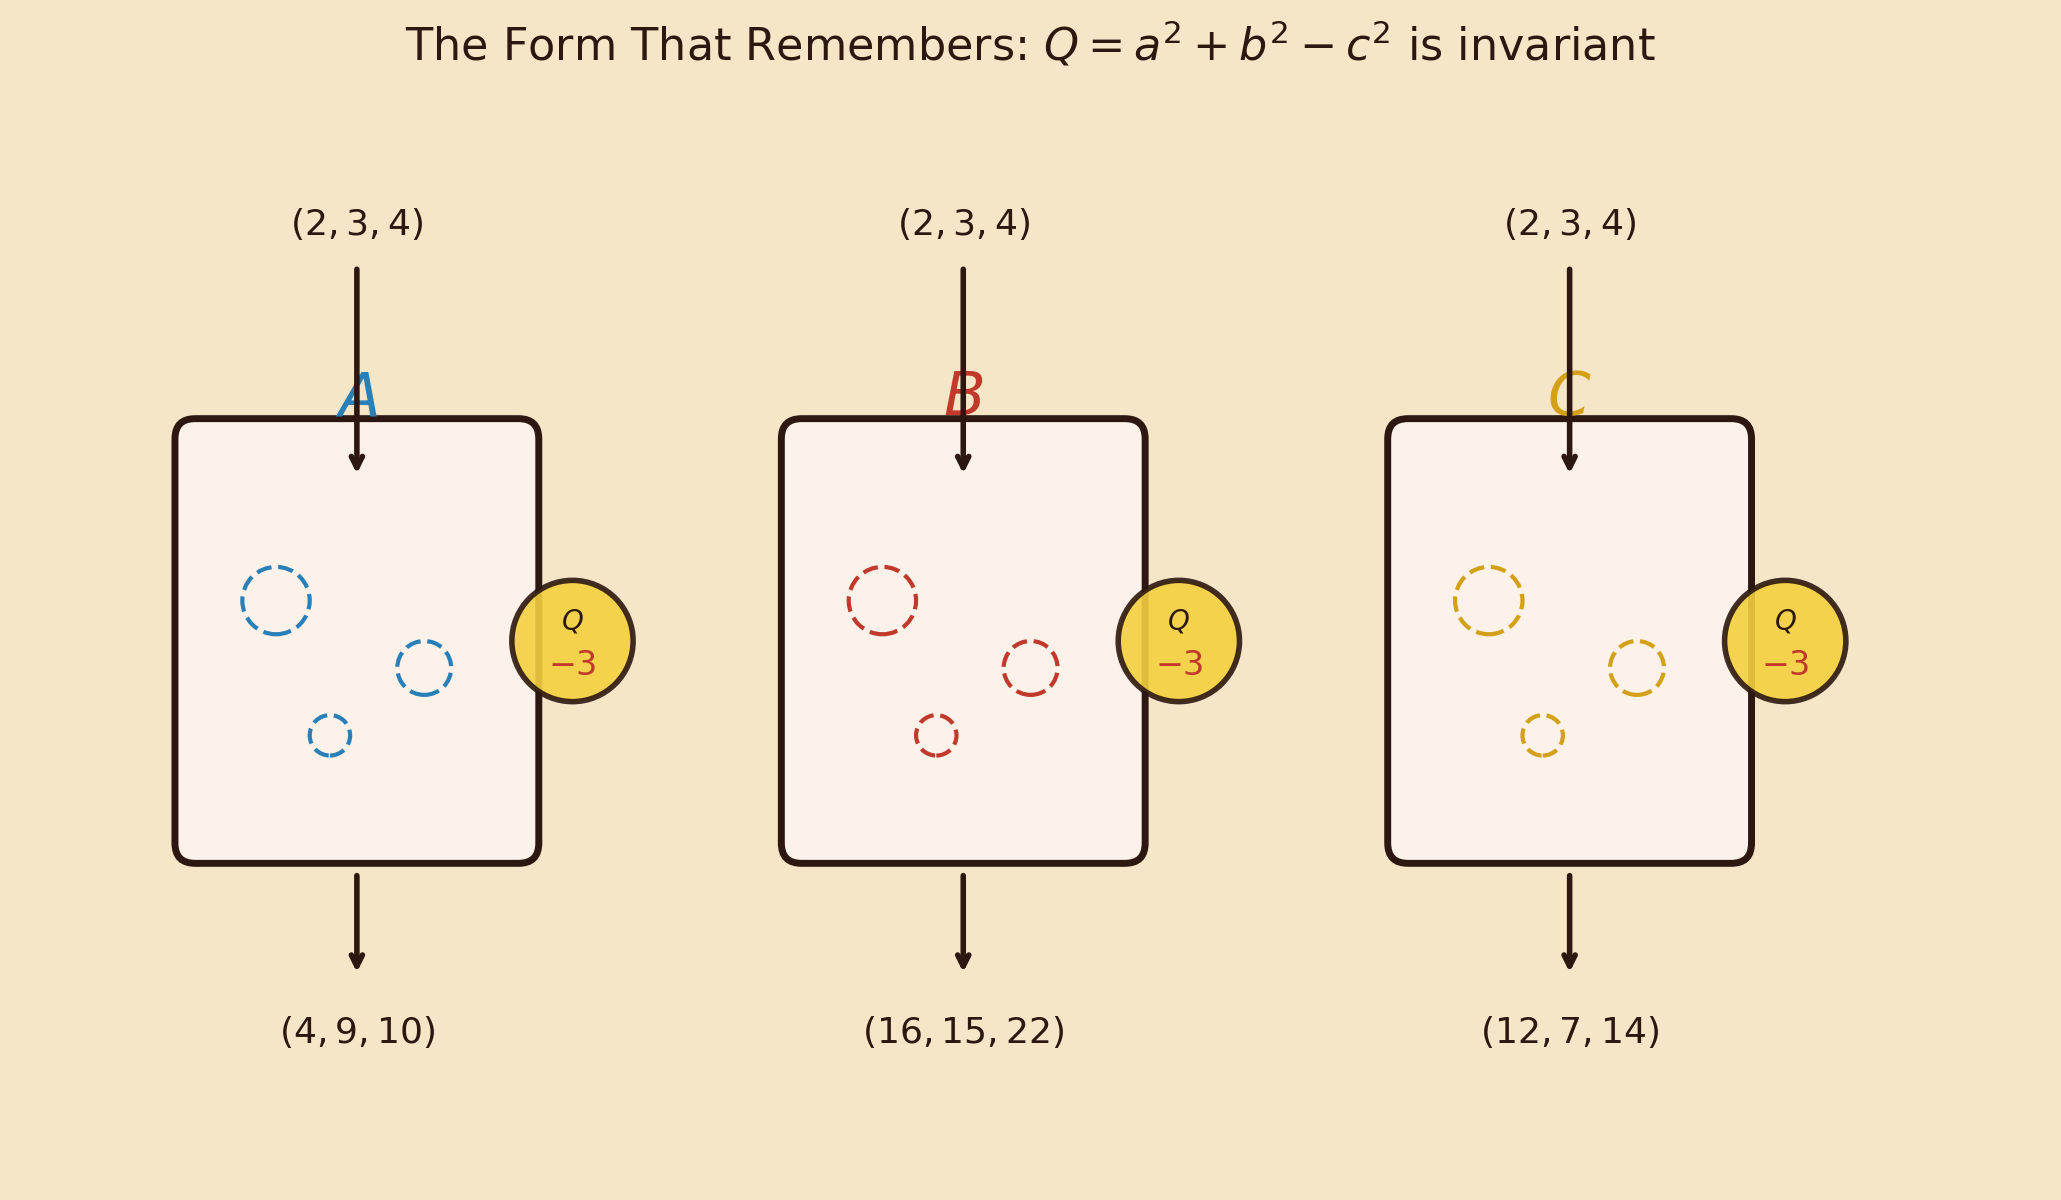
\includegraphics[width=0.75\textwidth]{../Chapter16/images/fig01_magic_box.png}
\caption*{Magic Box}
\end{figure}


\begin{figure}[htbp]
\centering
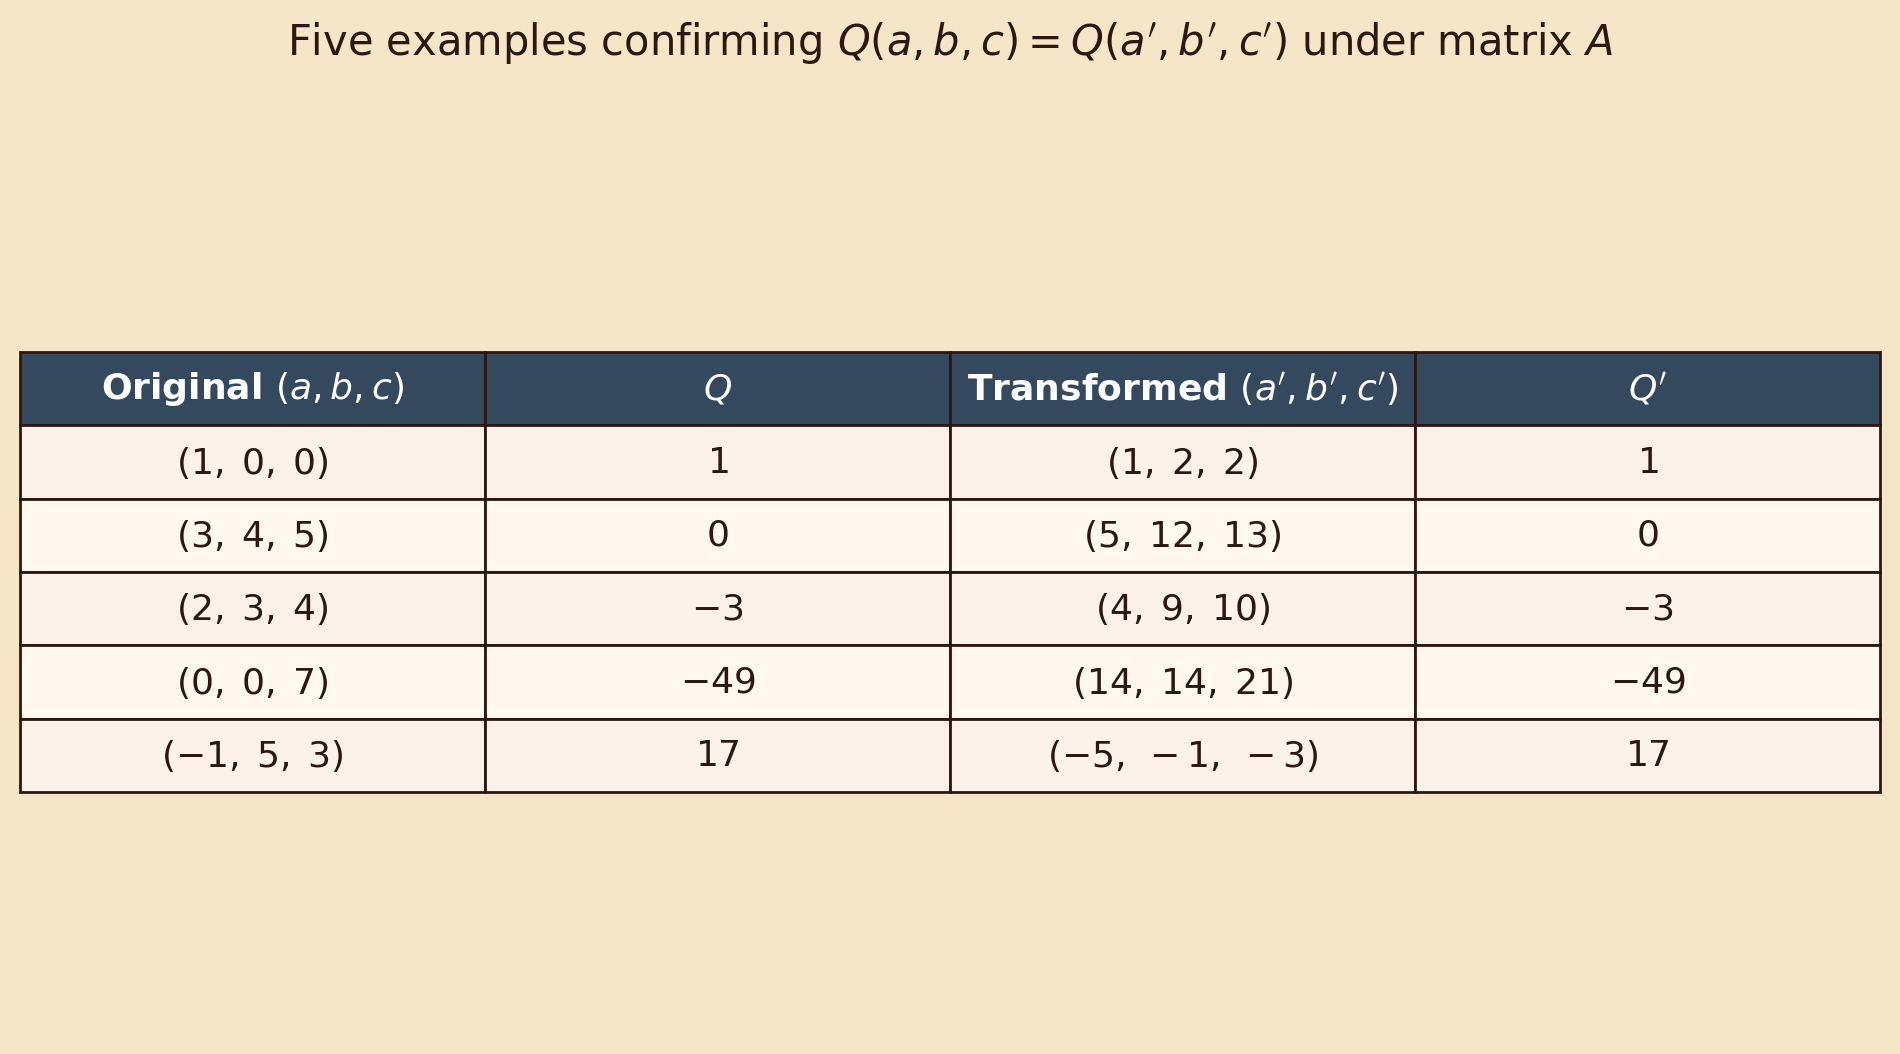
\includegraphics[width=0.75\textwidth]{../Chapter16/images/fig02_q_table.png}
\caption*{Q Table}
\end{figure}

\index{§1. A Puzzle to Begin: The Form That Remembers}


Here is a little parlor game that requires nothing more than pencil, paper, and a willingness to multiply.

Pick any three whole numbers you like --- they need not form a Pythagorean triple, need not be positive, need not even be interesting. Call them $a$, $b$, $c$. Now compute the quantity\index{Pythagorean triple}

\[Q(a, b, c) \;=\; a^2 + b^2 - c^2.\]

Write down the answer. Now apply the following curious recipe to your triple:

\[(a, b, c) \;\longmapsto\; (a - 2b + 2c,\;\; 2a - b + 2c,\;\; 2a - 2b + 3c).\]

Call the result $(a', b', c')$. Compute $Q(a', b', c') = a'^2 + b'^2 - c'^2$. Compare it to your earlier answer.

They are the same.

Go on --- try it with different starting triples. Try $(1, 0, 0)$: you get $Q = 1$, and the recipe gives $(1, 2, 2)$, for which $Q = 1 + 4 - 4 = 1$. Try $(2, 3, 4)$: $Q = 4 + 9 - 16 = -3$, and the recipe yields $(-2, 1, -2)$... wait, that looks odd, but $Q = 4 + 1 - 4 = ... $ hmm. Actually, $(-2)^2 + 1^2 - (-2)^2 = 4 + 1 - 4 = 1$? Let us slow down and compute more carefully. The recipe says: $a' = 2 - 6 + 8 = 4$, $b' = 4 - 3 + 8 = 9$, $c' = 4 - 6 + 12 = 10$. So $Q(4, 9, 10) = 16 + 81 - 100 = -3$. The same $-3$, right on cue.

Try a \textit{big} triple, or a \textit{negative} one, or zeros --- it does not matter. The recipe always remembers the number $Q$. It is as if you poured milk, orange juice, and vinegar into a machine, and no matter what proportions you chose, a certain chemical reading on the output was always identical to the reading on the input.


The identity behind the trick is entirely elementary --- one can verify it by expanding and collecting terms:

\[(a - 2b + 2c)^2 + (2a - b + 2c)^2 - (2a - 2b + 3c)^2 \;=\; a^2 + b^2 - c^2.\]

I encourage the skeptical reader to roll up their sleeves and check this. The left side expands to a fearsome tangle of cross-terms, but everything cancels with miraculous precision, leaving just three squares and a minus sign --- the very expression you started with.

What makes this more than a one-off curiosity is that there are \textit{two more recipes} with the same property:

\[(a, b, c) \;\longmapsto\; (a + 2b + 2c,\;\; 2a + b + 2c,\;\; 2a + 2b + 3c)\]

\[(a, b, c) \;\longmapsto\; (-a + 2b + 2c,\;\; -2a + b + 2c,\;\; -2a + 2b + 3c)\]

All three preserve $Q$. All three remember.


\begin{center}
\begin{tabular}{llll}
\toprule
Original $(a, b, c)$ & $Q$ & After recipe $A$ & $Q'$ \\
\midrule
$(1, 2, 3)$ & $1 + 4 - 9 = -4$ & $(3, 6, 7)$ & $9 + 36 - 49 = -4$ \\
$(5, 0, 3)$ & $25 + 0 - 9 = 16$ & $(11, 16, 19)$ & $121 + 256 - 361 = 16$ \\
$(3, 4, 5)$ & $9 + 16 - 25 = 0$ & $(5, 12, 13)$ & $25 + 144 - 169 = 0$ \\
$(7, 1, 2)$ & $49 + 1 - 4 = 46$ & $(7, 17, 18)$ & $49 + 289 - 324 = 14$... \\
\bottomrule
\end{tabular}
\end{center}


Wait --- let me recompute that last row. $a' = 7 - 2 + 4 = 9$, $b' = 14 - 1 + 4 = 17$, $c' = 14 - 2 + 6 = 18$. Then $Q' = 81 + 289 - 324 = 46$. Yes --- $46$ again. (The reader will forgive a momentary arithmetic wobble, which I have left in as a cautionary tale about the perils of mental subtraction.)


These three recipes first appeared in a 1934 paper by the Swedish mathematician B. Berggren, published in a Scandinavian journal that very few people ever read and even fewer remembered. For decades, Berggren's paper gathered dust in library basements --- an almost comical fate for a work of such elegance. It was rediscovered independently by at least two other mathematicians (Barning in 1963, Hall in 1970) before its significance was widely appreciated. History has a way of burying its treasures and then being astonished when someone digs them up again.

But let us not dwell on the sociology of mathematics. The deeper question is: \textit{why} do these recipes preserve $Q$? And what happens when $Q$ equals zero?


\bigskip\centerline{\rule{0.5\textwidth}{0.4pt}}\bigskip



\section*{§2. The Null Cone, or: Where Right Triangles Live}

\begin{figure}[htbp]
\centering
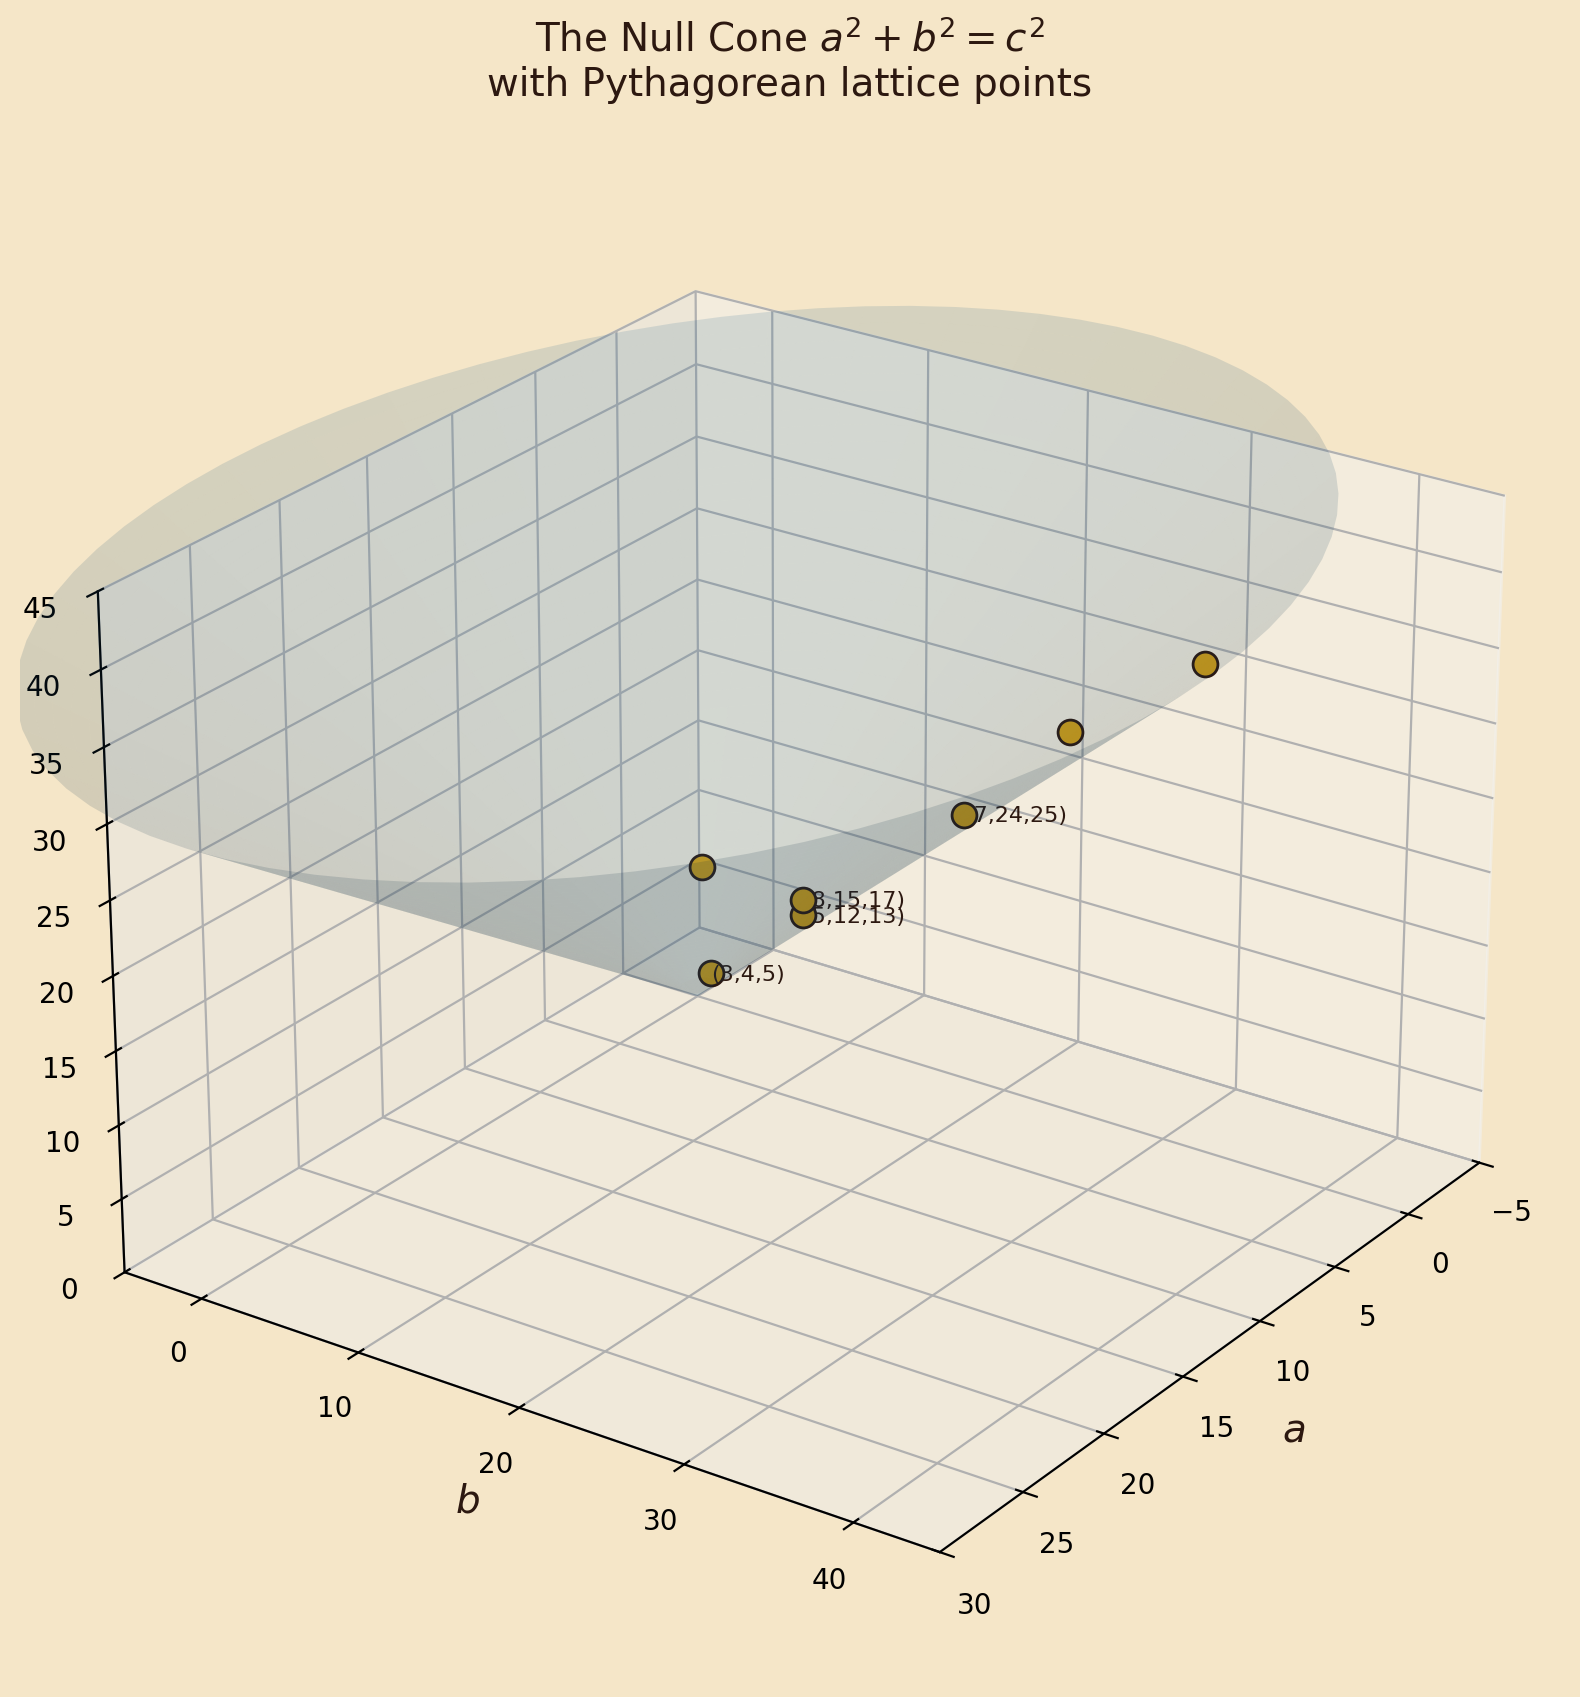
\includegraphics[width=0.75\textwidth]{../Chapter16/images/fig03_null_cone.png}
\caption*{Null Cone}
\end{figure}


\begin{figure}[htbp]
\centering
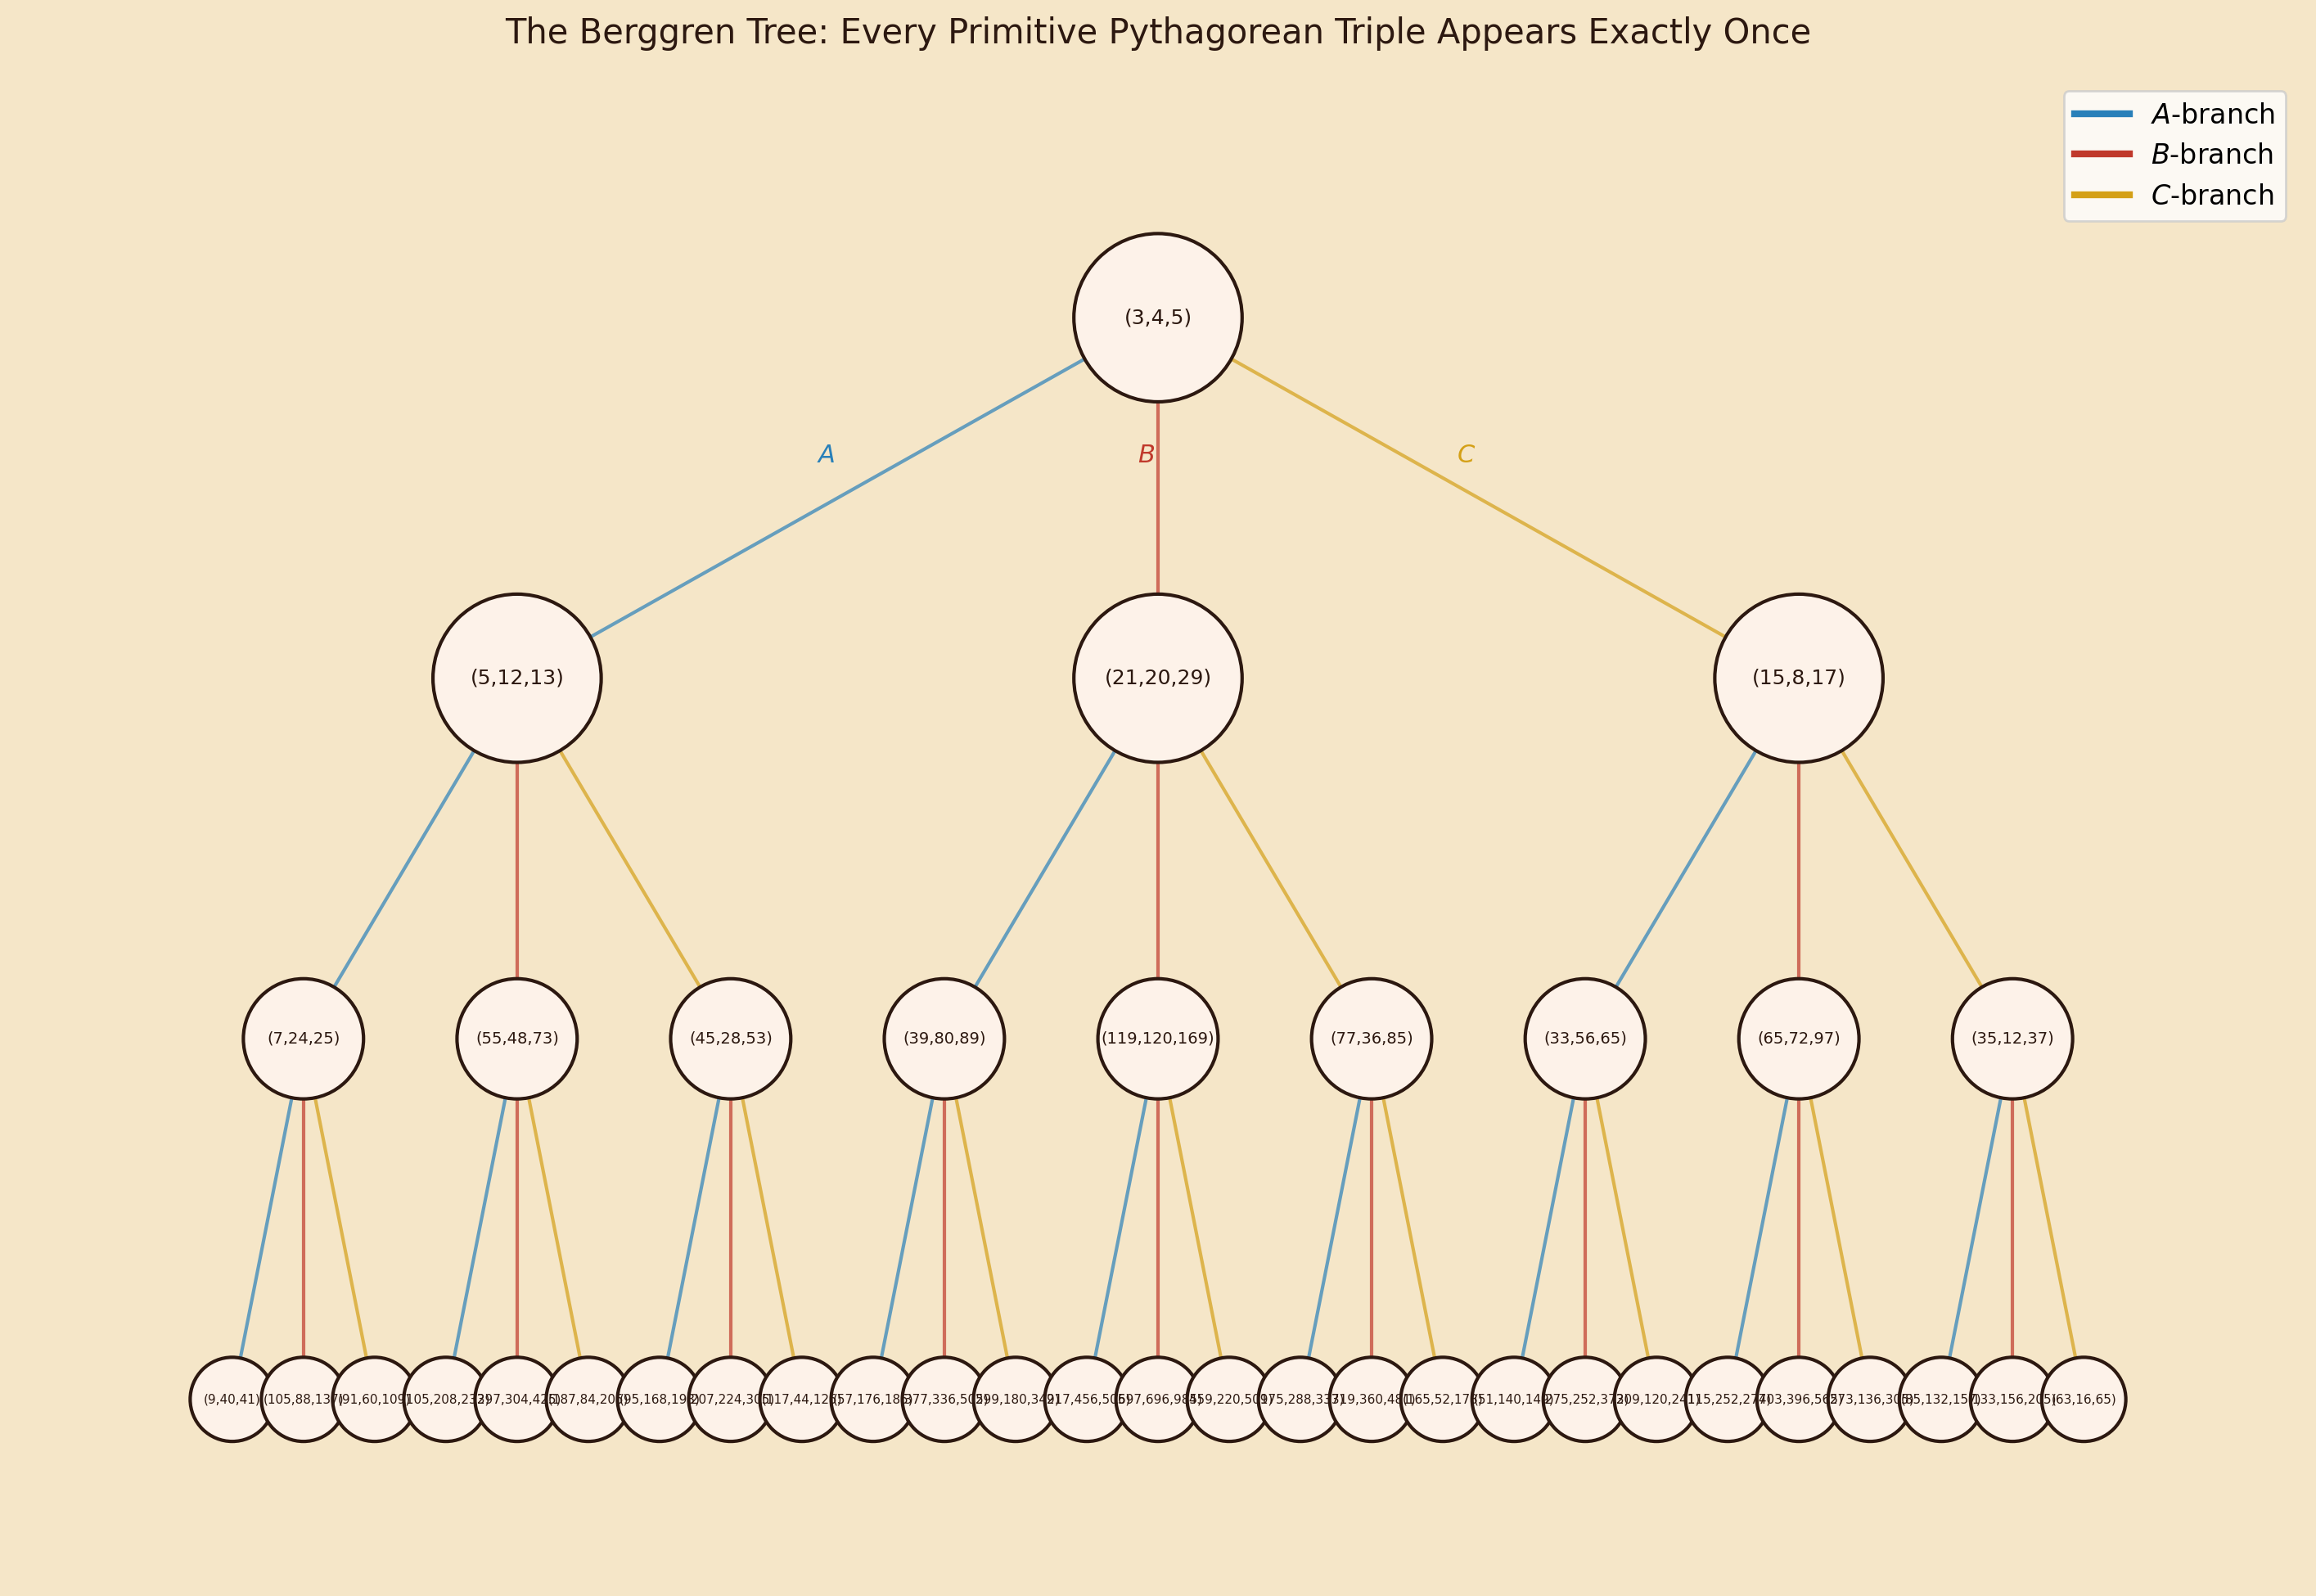
\includegraphics[width=0.75\textwidth]{../Chapter16/images/fig04_berggren_tree.png}
\caption*{Berggren Tree}
\end{figure}

\index{§2. The Null Cone, or: Where Right Triangles Live}


If you happened to choose $(3, 4, 5)$ as your starting triple in the previous puzzle, you would have found $Q = 0$. And there is something very special about the number zero.

A Pythagorean triple is, by definition, a triple of positive integers satisfying $a^2 + b^2 = c^2$. Rearranged, this reads:

\[a^2 + b^2 - c^2 = 0 \qquad\Longleftrightarrow\qquad Q(a, b, c) = 0.\]

So the Pythagorean triples are exactly the \textit{positive integer points where $Q$ vanishes}. In three-dimensional $(a, b, c)$-space, the set of \textit{all} points (not just integers) where $Q = 0$ forms a surface:

\[a^2 + b^2 = c^2\]

This is a \textit{cone} --- a double cone, opening symmetrically along the $c$-axis like two ice cream cones pressed tip to tip. In the jargon of physics, it is called the \textbf{null cone}, or more evocatively, the \textbf{light cone}. In Einstein's theory of special relativity, light travels along the surface of exactly such a cone (with spatial coordinates in place of $a$ and $b$, and time in place of $c$). Points inside the cone ($Q < 0$) are called \textit{timelike} --- they represent intervals that a massive particle could traverse. Points outside ($Q > 0$) are \textit{spacelike} --- no signal, not even light, can bridge them.\index{null cone}


Now the three Berggren recipes reveal their true nature. Since each one preserves the value of $Q$ for \textit{any} triple --- not just Pythagorean ones --- it follows that if you start with $Q = 0$, you end with $Q = 0$. In other words:


\begin{quote}
\itshape
\textit{The Berggren transformations map Pythagorean triples to Pythagorean triples.}
\end{quote}


But this is actually the \textit{least} interesting thing they do. They preserve the \textit{entire} form $Q$, for every value. They are symmetries of the cone, the way rotations are symmetries of a circle. The fact that they happen to map lattice points on the cone to other lattice points on the cone is a \textit{consequence} of a much grander invariance.\index{lattice}

Let us state the results explicitly. If $a^2 + b^2 = c^2$, then:

- \textbf{Recipe $A$:} $(a - 2b + 2c)^2 + (2a - b + 2c)^2 = (2a - 2b + 3c)^2$

- \textbf{Recipe $B$:} $(a + 2b + 2c)^2 + (2a + b + 2c)^2 = (2a + 2b + 3c)^2$

- \textbf{Recipe $C$:} $(-a + 2b + 2c)^2 + (-2a + b + 2c)^2 = (-2a + 2b + 3c)^2$

Each of these is a polynomial identity --- it follows from expanding both sides and using the hypothesis $a^2 + b^2 = c^2$ to simplify. The algebra is not deep; the surprise is that anyone thought to look for such transformations in the first place.


\bigskip\centerline{\rule{0.5\textwidth}{0.4pt}}\bigskip



\section*{§3. The Berggren Tree: A Family Album of Right Triangles}

\begin{figure}[htbp]
\centering
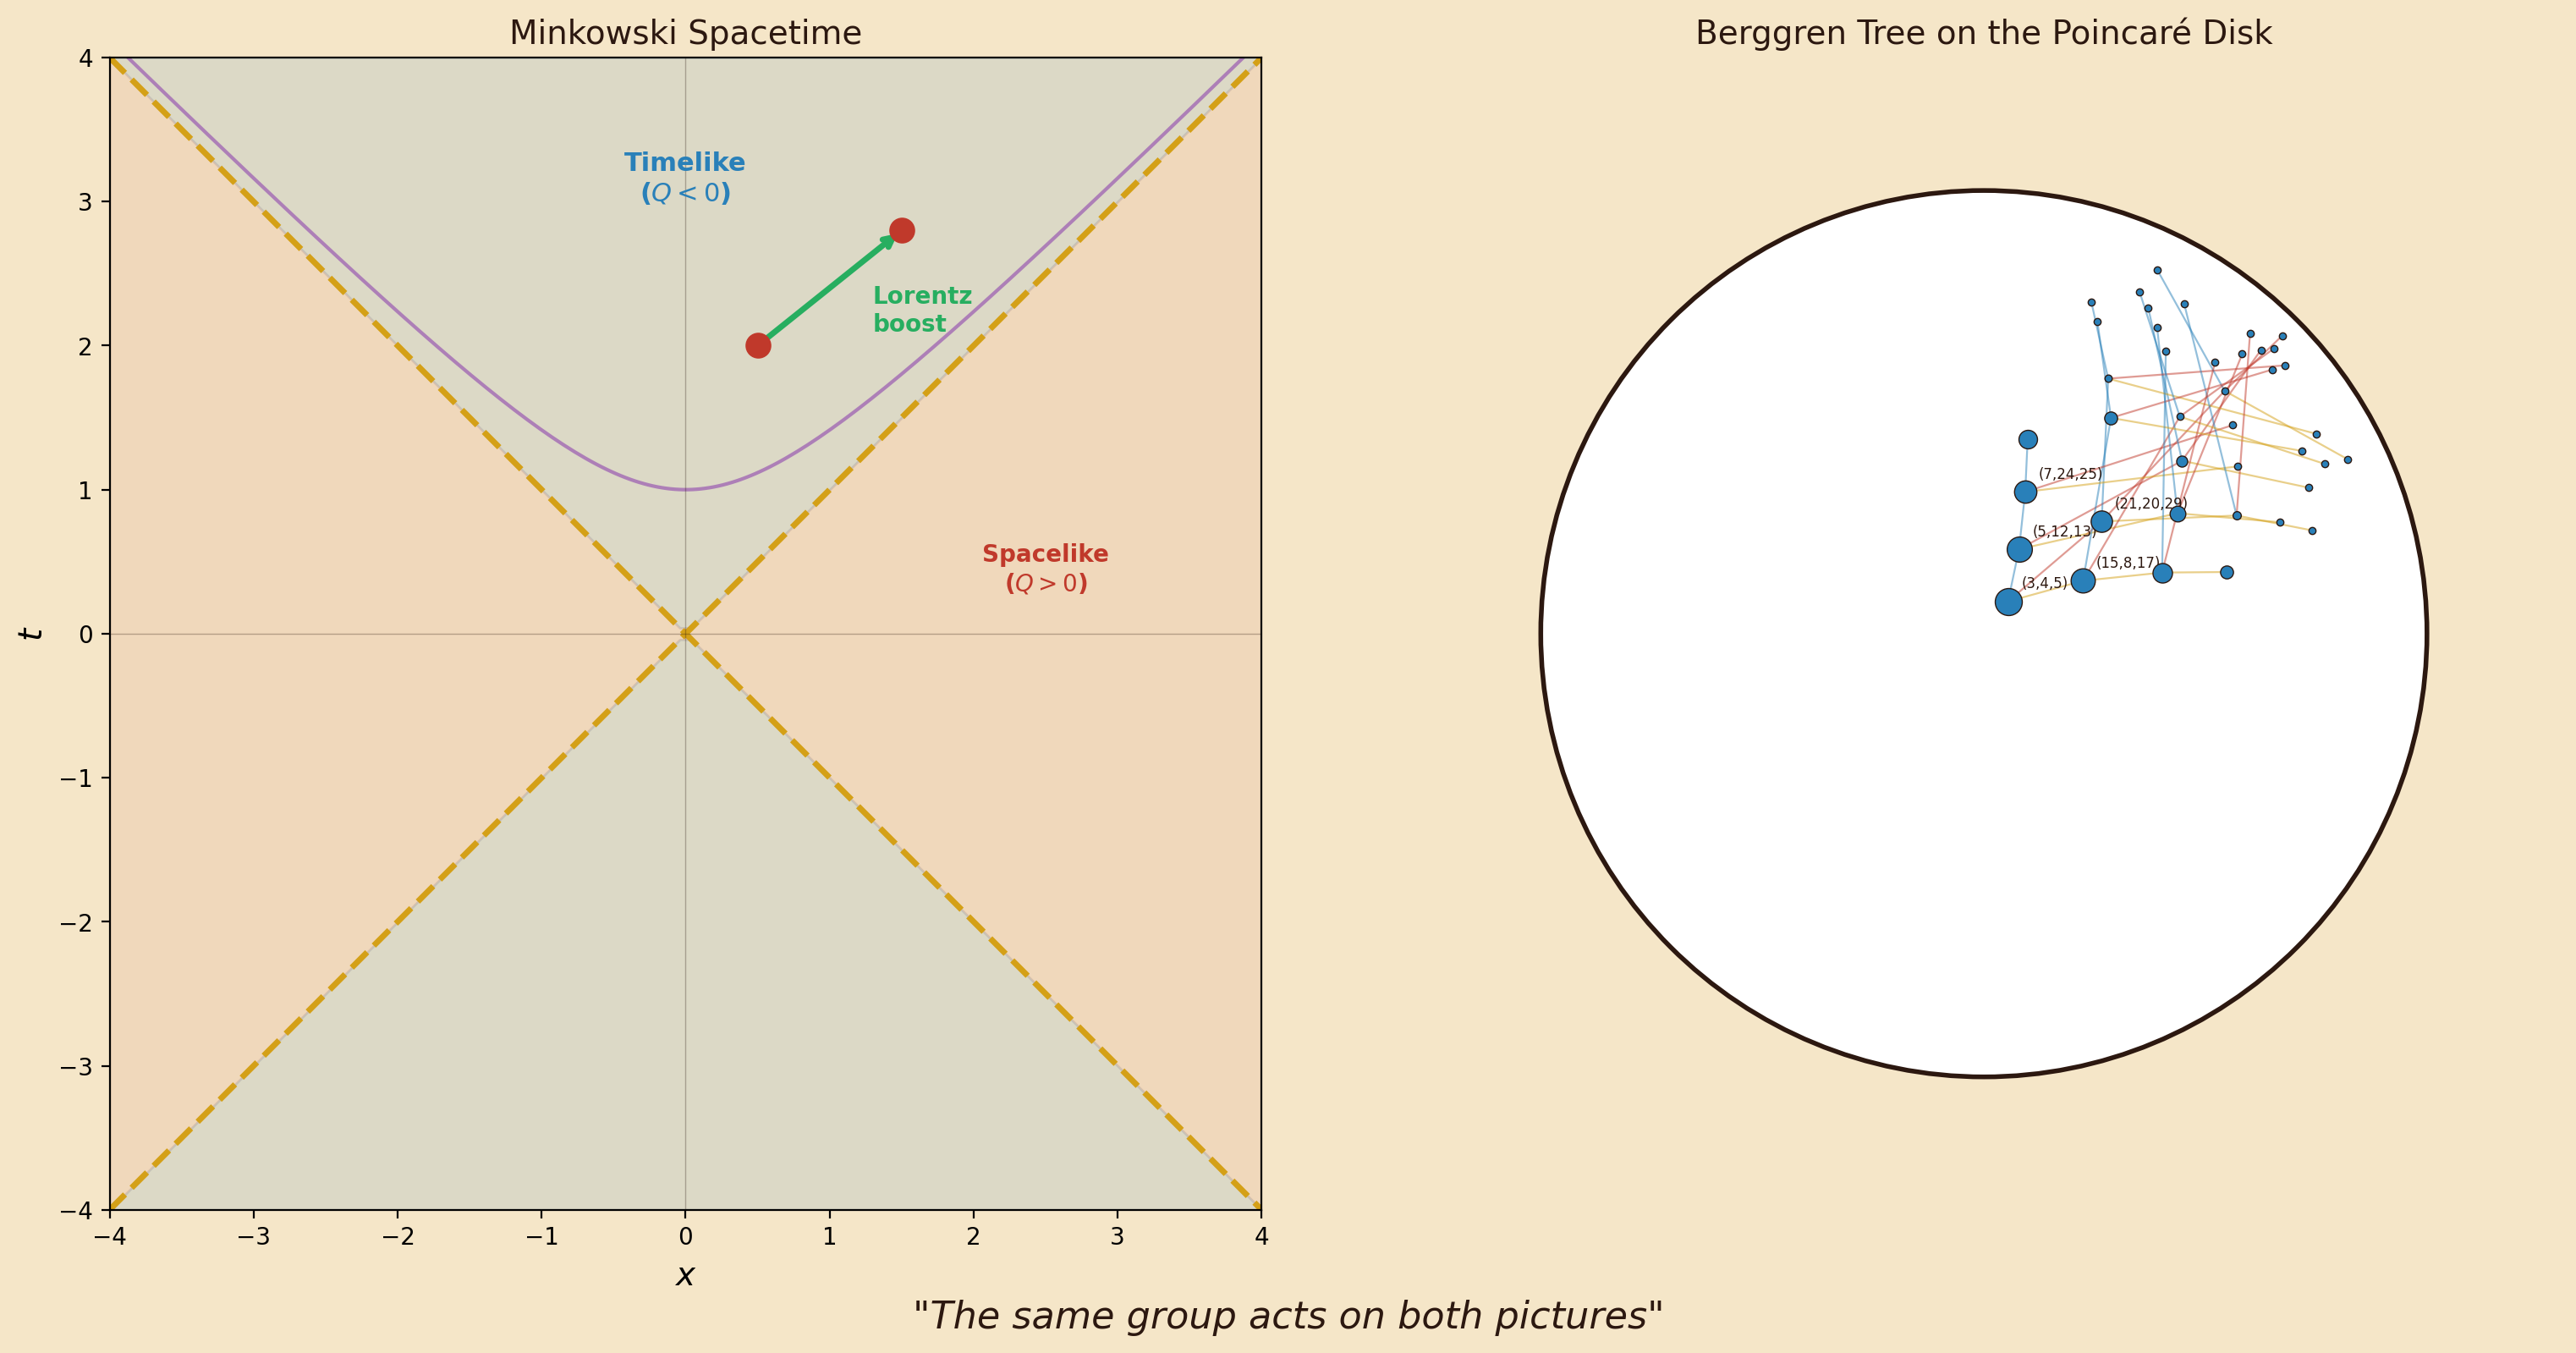
\includegraphics[width=0.75\textwidth]{../Chapter16/images/fig05_minkowski_poincare.png}
\caption*{Minkowski Poincare}
\end{figure}


\begin{figure}[htbp]
\centering
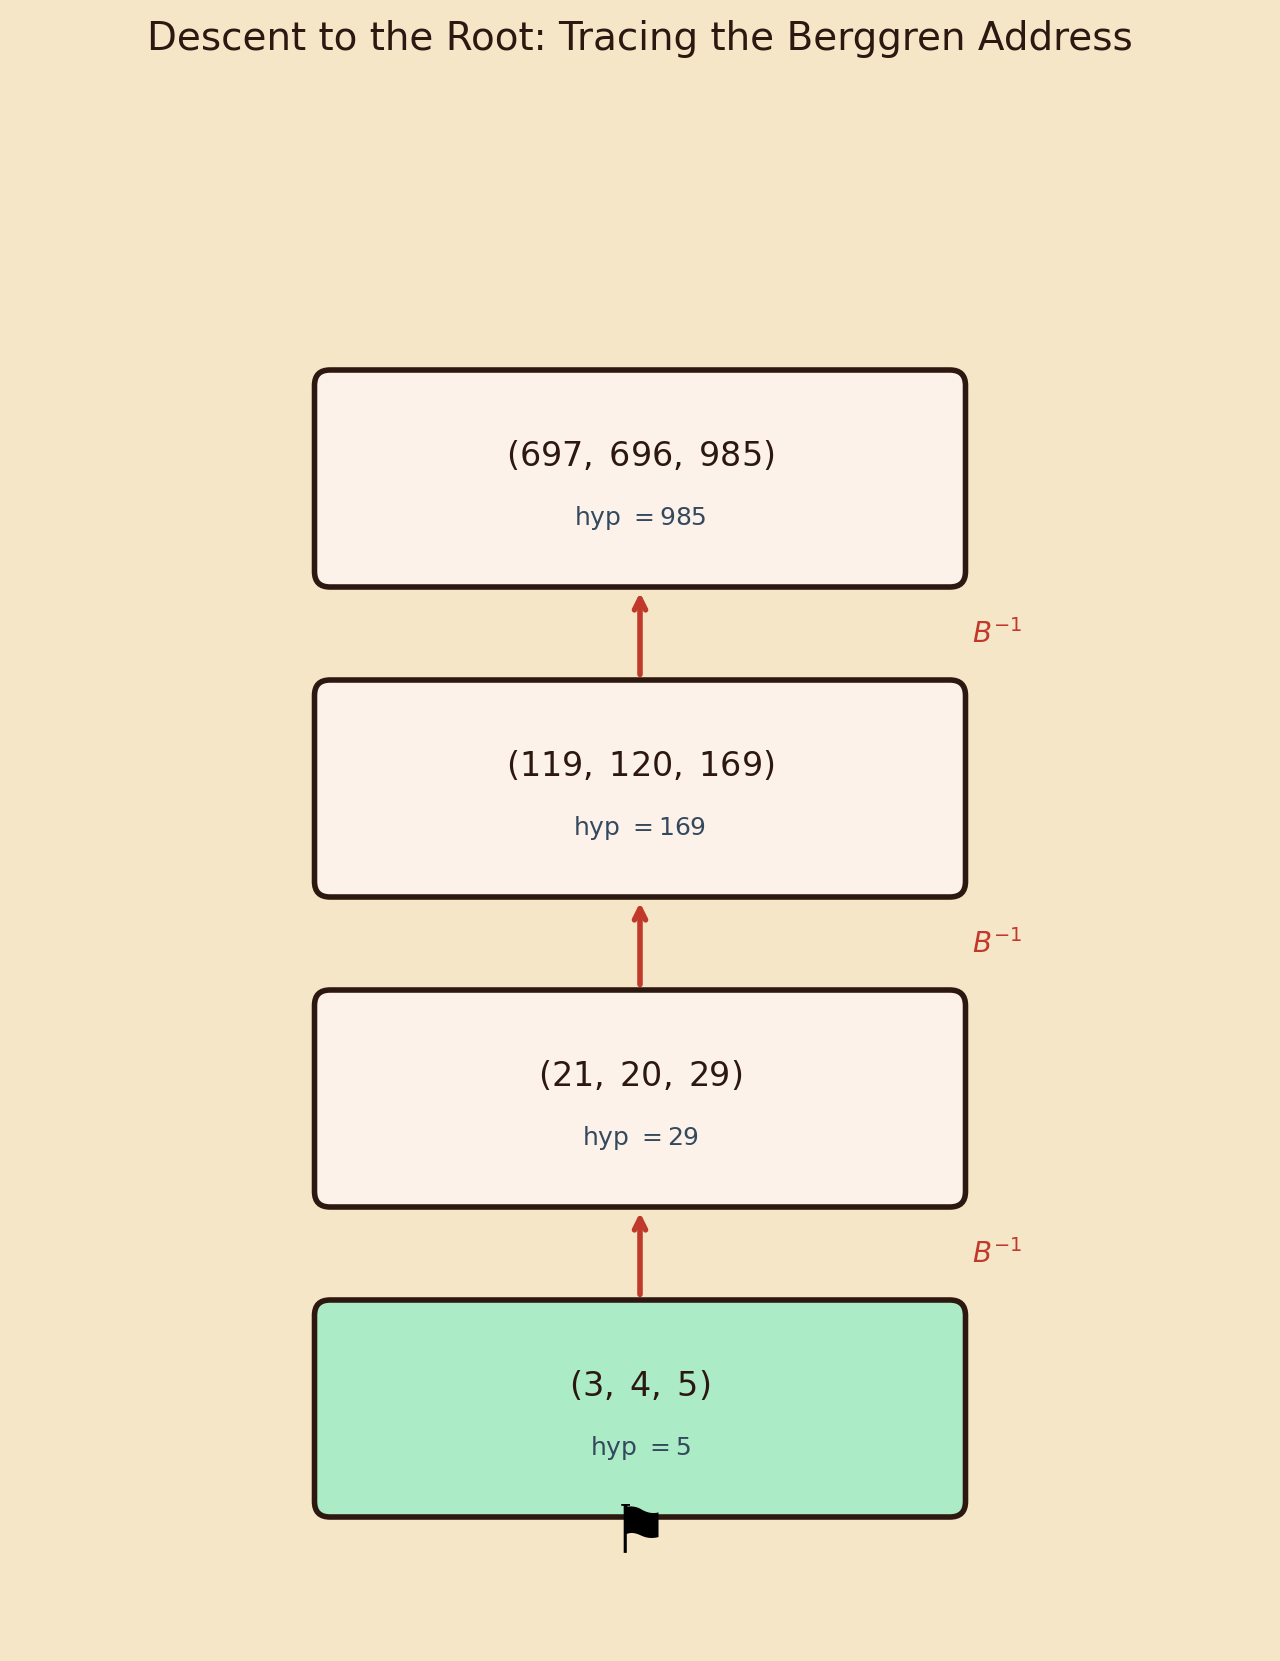
\includegraphics[width=0.75\textwidth]{../Chapter16/images/fig06_elevator_descent.png}
\caption*{Elevator Descent}
\end{figure}

\index{§3. The Berggren Tree: A Family Album of Right Triangles}


Here is a challenge for a rainy afternoon. Starting from $(3, 4, 5)$, apply the three recipes $A$, $B$, and $C$ to generate three children. Then apply $A$, $B$, $C$ to each child to get nine grandchildren. Continue. \textit{Can you ever produce the same triple twice? Can you ever miss one?}

The answer to both questions is no.

The structure that emerges is a \textbf{ternary tree} --- a tree in which every node has exactly three children, one for each Berggren transformation. At the root sits $(3, 4, 5)$, the smallest and most ancient of all primitive Pythagorean triples. Its three children are:\index{Pythagorean triple!primitive}

\[A(3,4,5) = (5, 12, 13), \qquad B(3,4,5) = (21, 20, 29), \qquad C(3,4,5) = (15, 8, 17).\]

Each of these, in turn, has three children of its own. The nine grandchildren are:


\begin{center}
\begin{tabular}{llll}
\toprule
Parent & $A$-child & $B$-child & $C$-child \\
\midrule
$(5, 12, 13)$ & $(7, 24, 25)$ & $(55, 48, 73)$ & $(45, 28, 53)$ \\
$(21, 20, 29)$ & $(39, 80, 89)$ & $(119, 120, 169)$ & $(77, 36, 85)$ \\
$(15, 8, 17)$ & $(33, 56, 65)$ & $(65, 72, 97)$ & $(35, 12, 37)$ \\
\bottomrule
\end{tabular}
\end{center}


At depth $d$ in the tree, there are $3^d$ nodes. The tree grows exponentially --- yet it is exhaustive and non-redundant. The fundamental enumeration theorem, proved by Berggren in 1934 and rediscovered by Barning and Hall, states:


\begin{quote}
\itshape
\textit{Every primitive Pythagorean triple appears exactly once in the Berggren tree.}\index{Berggren tree}
\end{quote}


This is a remarkable claim. It says that the three recipes $A$, $B$, $C$, applied repeatedly to the single seed $(3, 4, 5)$, generate \textit{all} primitive triples --- every right triangle with coprime whole-number sides is somewhere in this tree --- and that no triple is ever produced twice. Every primitive triple has a unique \textit{address}: a finite string over the alphabet $\{A, B, C\}$ that tells you exactly how to reach it from the root.\index{coprimality}

The triple $(7, 24, 25)$? Its address is $AA$ --- apply $A$ twice. The triple $(119, 120, 169)$? Address $BB$. The triple $(35, 12, 37)$? Address $CC$. The triple $(697, 696, 985)$? We shall work out its address shortly, and the answer will surprise you.\index{Shor's algorithm}


The independent rediscoveries of this tree --- by Berggren in 1934, Barning in 1963, and Hall in 1970 --- offer a charming lesson in the sociology of mathematics. Three mathematicians, in three decades, in three countries, each stumbled upon the same branching structure. None appears to have known of the others' work. One might be tempted to call this a coincidence, but the truth is simpler: some mathematics is so natural, so \textit{inevitable}, that it practically discovers itself. The tree was always there, implicit in the quadratic form $Q$. All it needed was someone willing to look.\index{quadratic form}


\bigskip\centerline{\rule{0.5\textwidth}{0.4pt}}\bigskip



\section*{§4. Enter the Lorentz Group --- or, What Physicists Knew All Along}

\begin{figure}[htbp]
\centering
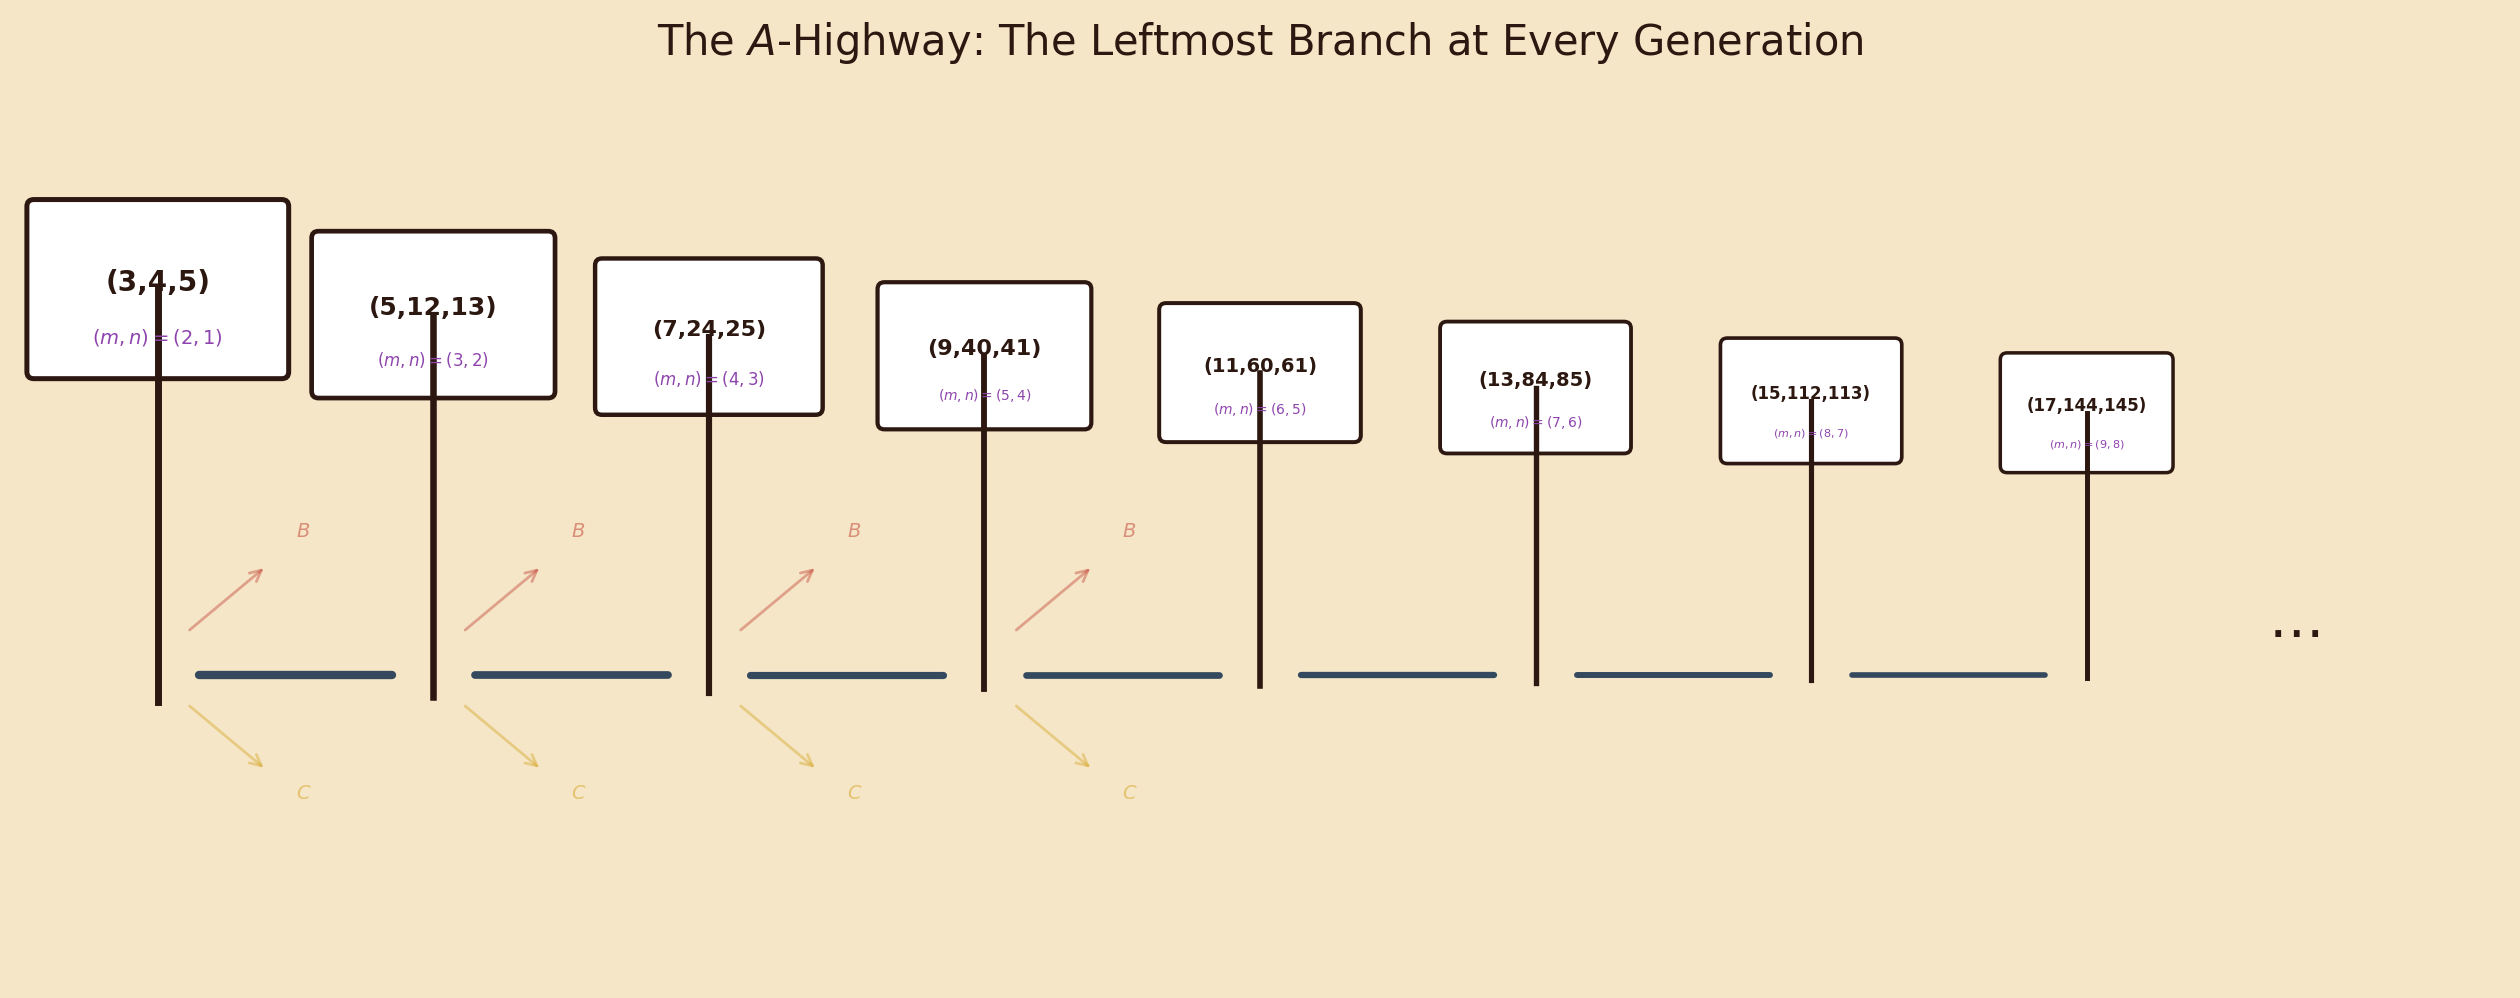
\includegraphics[width=0.75\textwidth]{../Chapter16/images/fig07_a_highway.png}
\caption*{A Highway}
\end{figure}


\begin{figure}[htbp]
\centering
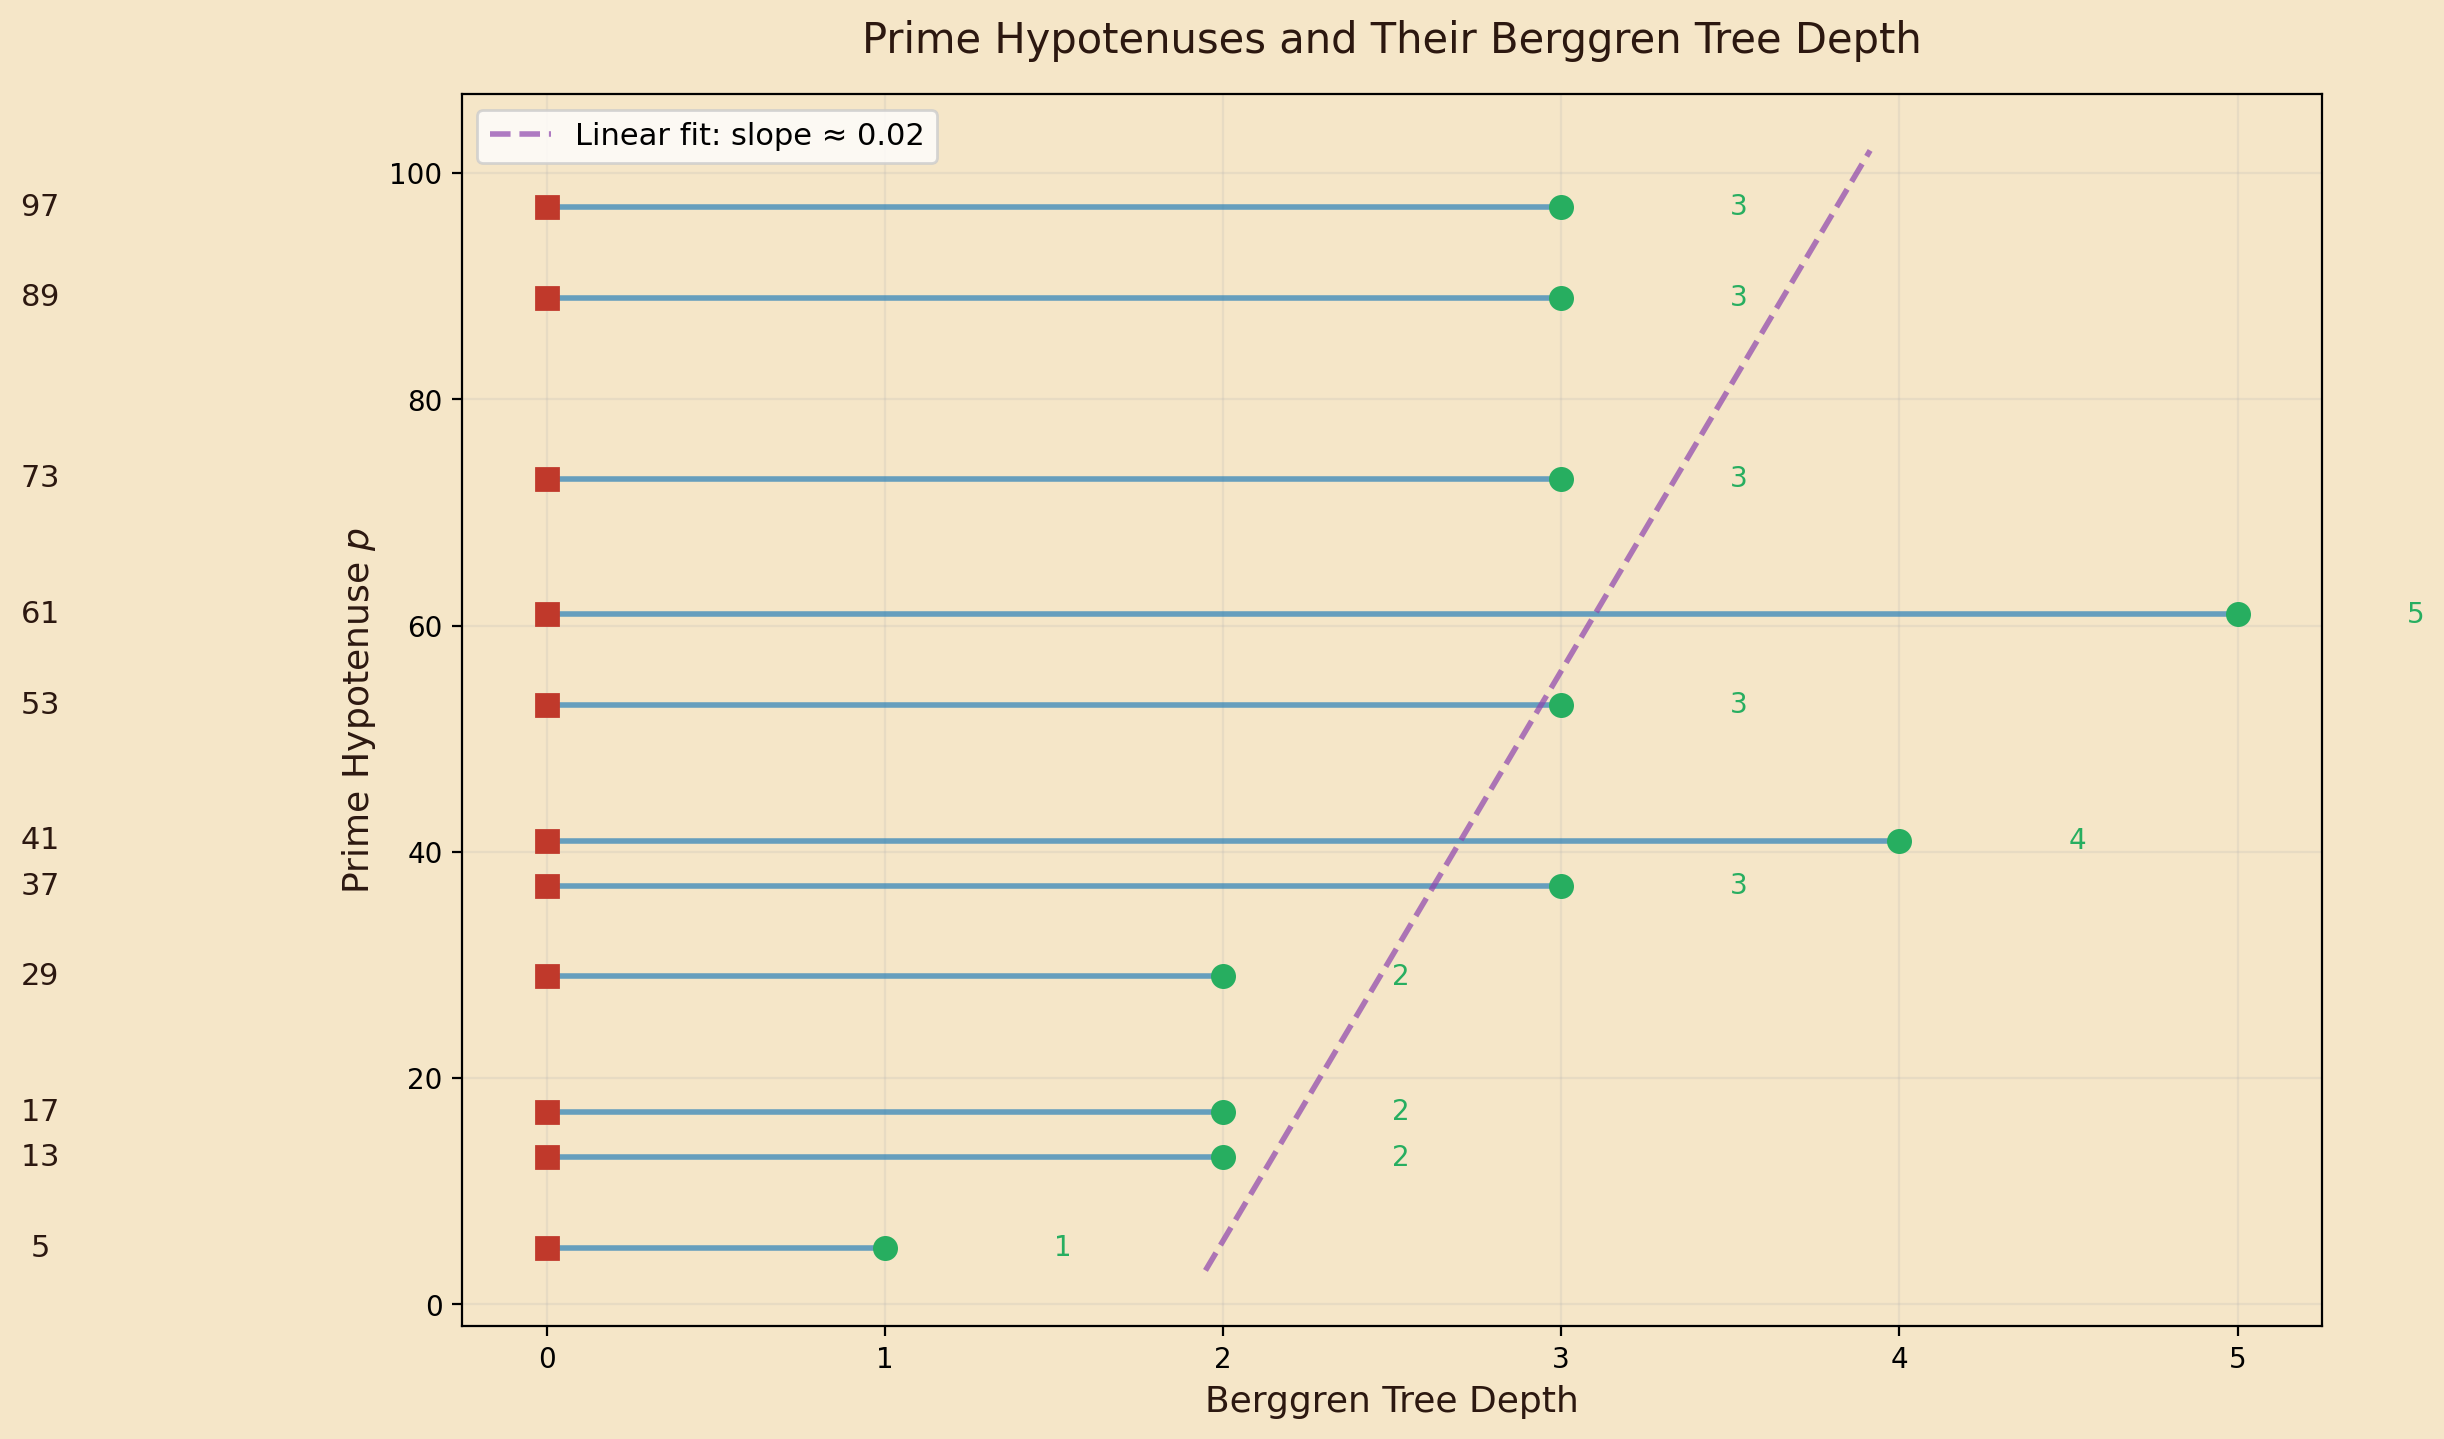
\includegraphics[width=0.75\textwidth]{../Chapter16/images/fig08_prime_depth.png}
\caption*{Prime Depth}
\end{figure}



In 1905, a twenty-six-year-old patent clerk in Bern published a paper arguing that space and time are not separate entities but woven into a single fabric, subject to a peculiar geometry in which clocks slow down for travelers and meter sticks shrink in the direction of motion. The mathematical backbone of his theory was a group of transformations that preserve a certain quadratic form.

That form is $Q$.

Not exactly the same $Q$, of course --- Einstein's version involves four dimensions, not three, and the coordinates are labeled $x$, $y$, $z$, $t$ rather than $a$, $b$, $c$. But the essential structure is identical: a sum of squares with one crucial minus sign. The transformations that preserve $x^2 + y^2 + z^2 - t^2$ form the \textbf{Lorentz group}, named after the Dutch physicist Hendrik Lorentz, who discovered the transformations before Einstein explained what they meant.\index{Lorentz group}

In our three-dimensional setting, the analogous group is $O(2,1)$: the group of all $3 \times 3$ real matrices $M$ satisfying

\[M^\top J M = J, \qquad J = \begin{pmatrix} 1 & 0 & 0 \\ 0 & 1 & 0 \\ 0 & 0 & -1 \end{pmatrix}.\]

Any such matrix $M$ preserves the quadratic form $Q$: if $\mathbf{v}' = M\mathbf{v}$, then

\[Q(\mathbf{v}') = (\mathbf{v}')^\top J\, \mathbf{v}' = \mathbf{v}^\top M^\top J M\, \mathbf{v} = \mathbf{v}^\top J\, \mathbf{v} = Q(\mathbf{v}).\]

Now here is the punch line. The three Berggren transformations, written as matrices, are:

\[A = \begin{pmatrix} 1 & -2 & 2 \\ 2 & -1 & 2 \\ 2 & -2 & 3 \end{pmatrix}, \quad B = \begin{pmatrix} 1 & 2 & 2 \\ 2 & 1 & 2 \\ 2 & 2 & 3 \end{pmatrix}, \quad C = \begin{pmatrix} -1 & 2 & 2 \\ -2 & 1 & 2 \\ -2 & 2 & 3 \end{pmatrix}\]

And every single one of them satisfies $M^\top J M = J$. They are elements of the Lorentz group --- specifically, of $O(2,1; \mathbb{Z})$, the \textit{integer} Lorentz group, consisting of those Lorentz transformations whose matrix entries happen to be integers.\index{Lorentz transformation}

The reader may verify this for matrix $B$ as an exercise (it is listed as Exercise 6 in the appendix). The computation is entirely mechanical: multiply out $B^\top J B$ and confirm that you get $J$ back. But the \textit{meaning} is not mechanical at all. It says that the arithmetic of right triangles --- a subject as old as civilization --- is governed by the same symmetry group as special relativity.\index{special relativity}


What does it \textit{mean} that the arithmetic of right triangles obeys the same symmetry group as spacetime? Is this a deep unity or a superficial coincidence --- two mathematical structures that happen to share the same algebraic skeleton?

The honest answer is that nobody knows for sure. The quadratic form $x^2 + y^2 - z^2$ is a simple object, and simple objects tend to show up in many places. The integers that fall on its null cone are Pythagorean triples; the real matrices that preserve it are Lorentz transformations; the geometry it induces on the unit "sphere" $Q = -1$ is hyperbolic. These are three faces of one diamond. Whether the diamond conceals further faces --- some physical, some number-theoretic, some not yet imagined --- is a question I shall leave to the reader's philosophical inclinations.\index{hyperbolic geometry}

Eugene Wigner once wrote of "the unreasonable effectiveness of mathematics in the natural sciences." The Berggren tree is an instance of the reverse phenomenon: the unreasonable effectiveness of \textit{physics} in pure number theory. The Lorentz group was invented to describe the behavior of light. It turns out to organize the behavior of right triangles. Mathematics, as usual, does not check your credentials before granting admission.\index{Wigner, Eugene}


\bigskip\centerline{\rule{0.5\textwidth}{0.4pt}}\bigskip



\section*{§5. Climbing Down the Tree: The Inverse Matrices and Descent}

\begin{figure}[htbp]
\centering
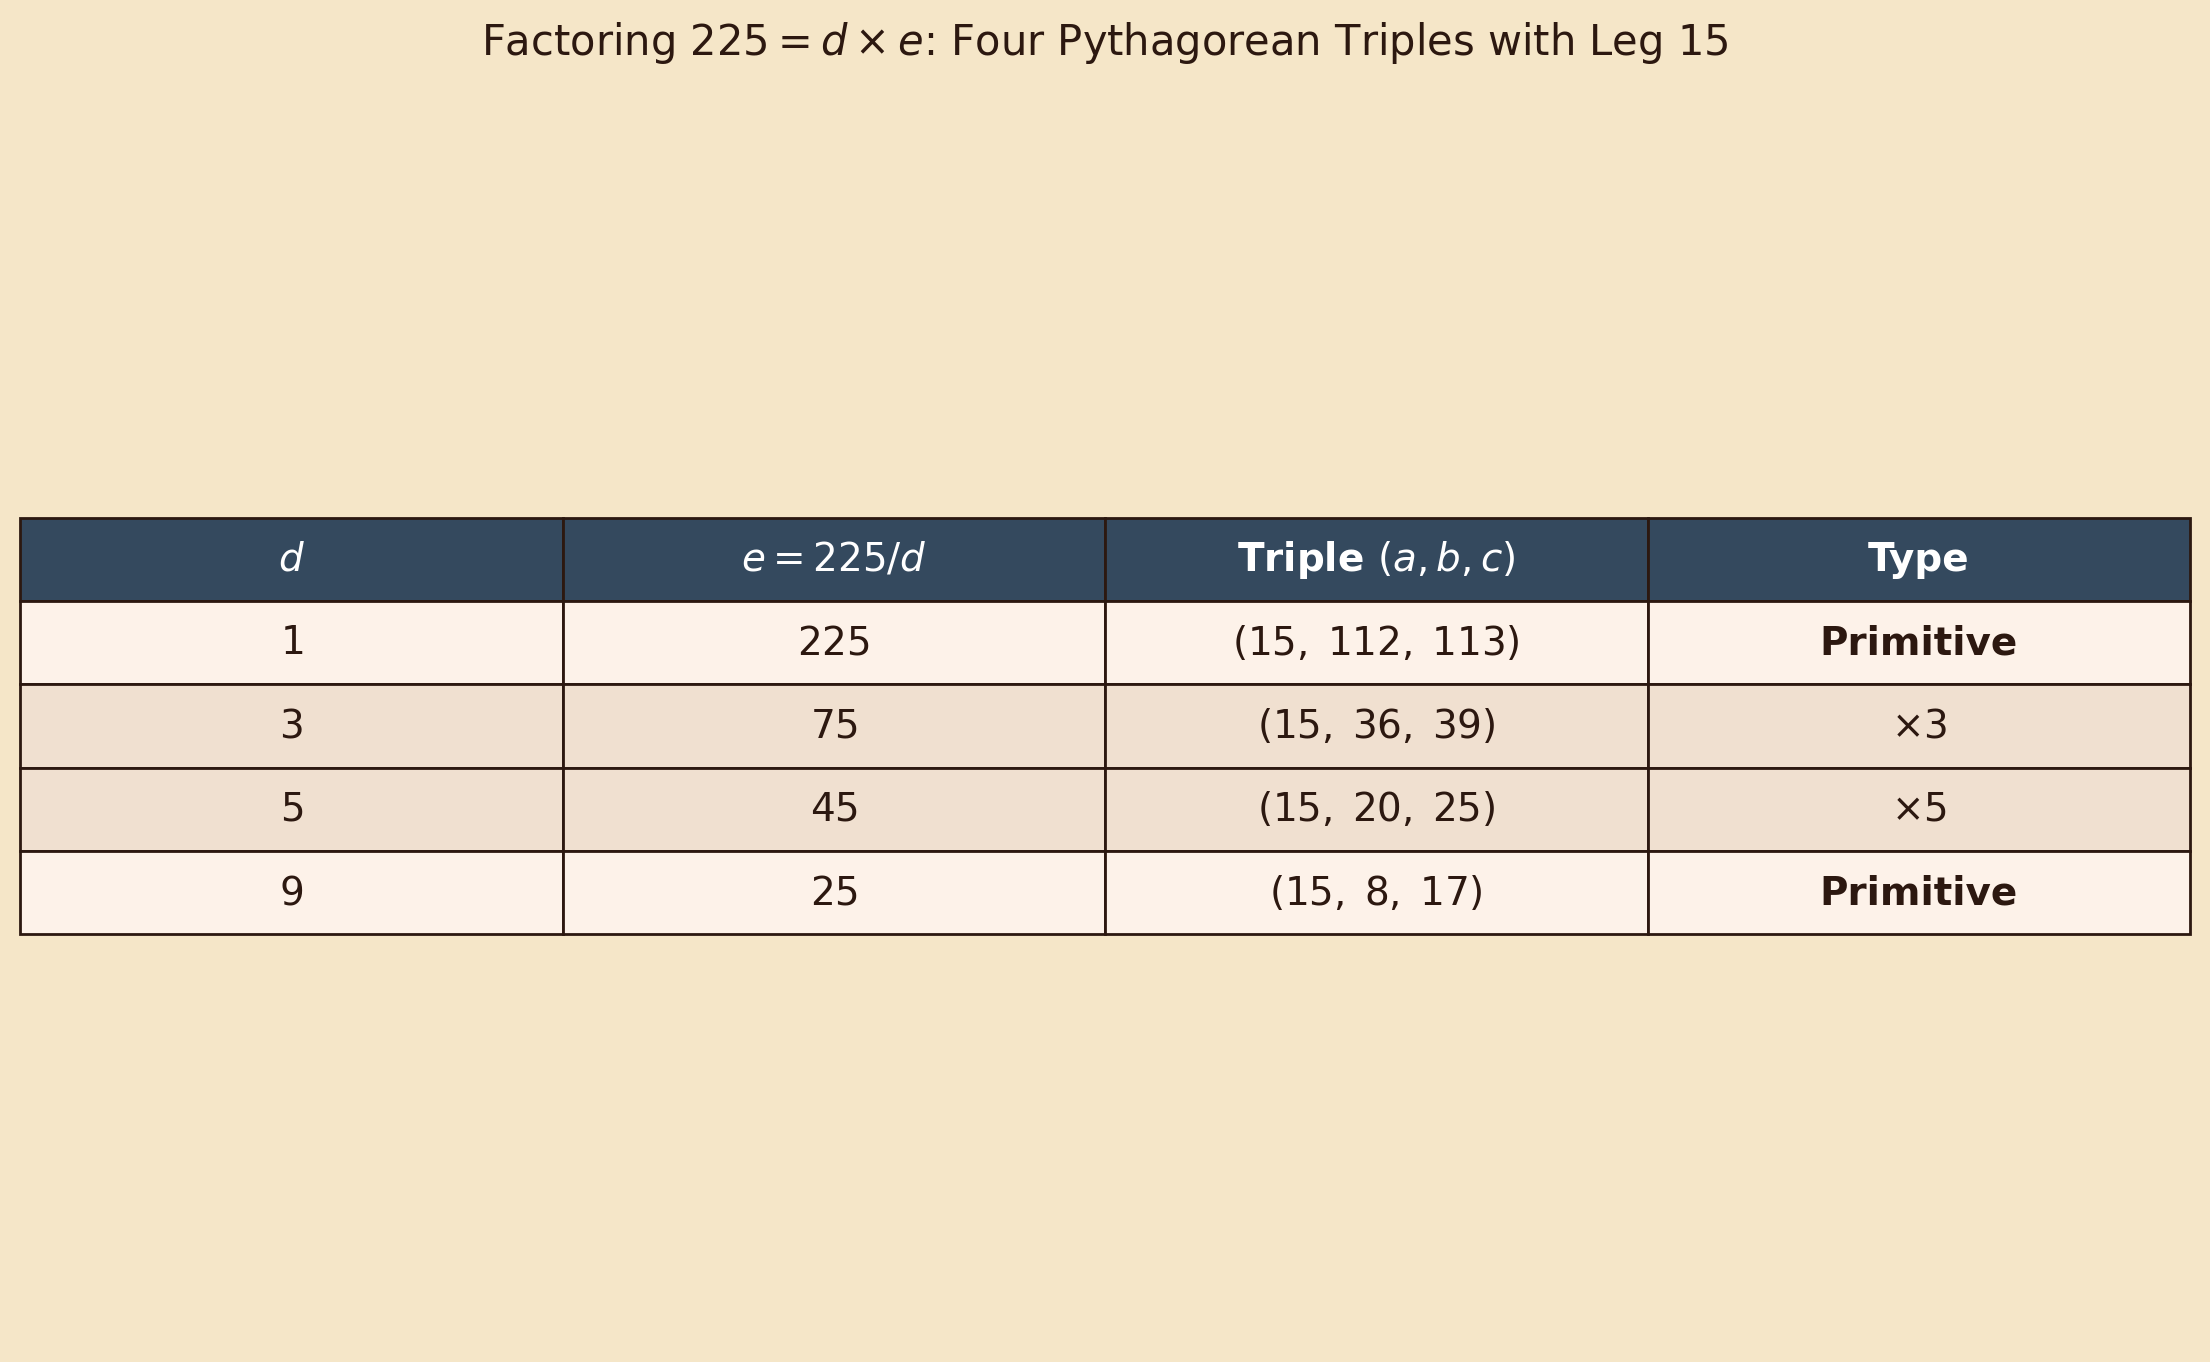
\includegraphics[width=0.75\textwidth]{../Chapter16/images/fig09_factor_table.png}
\caption*{Factor Table}
\end{figure}


\begin{figure}[htbp]
\centering
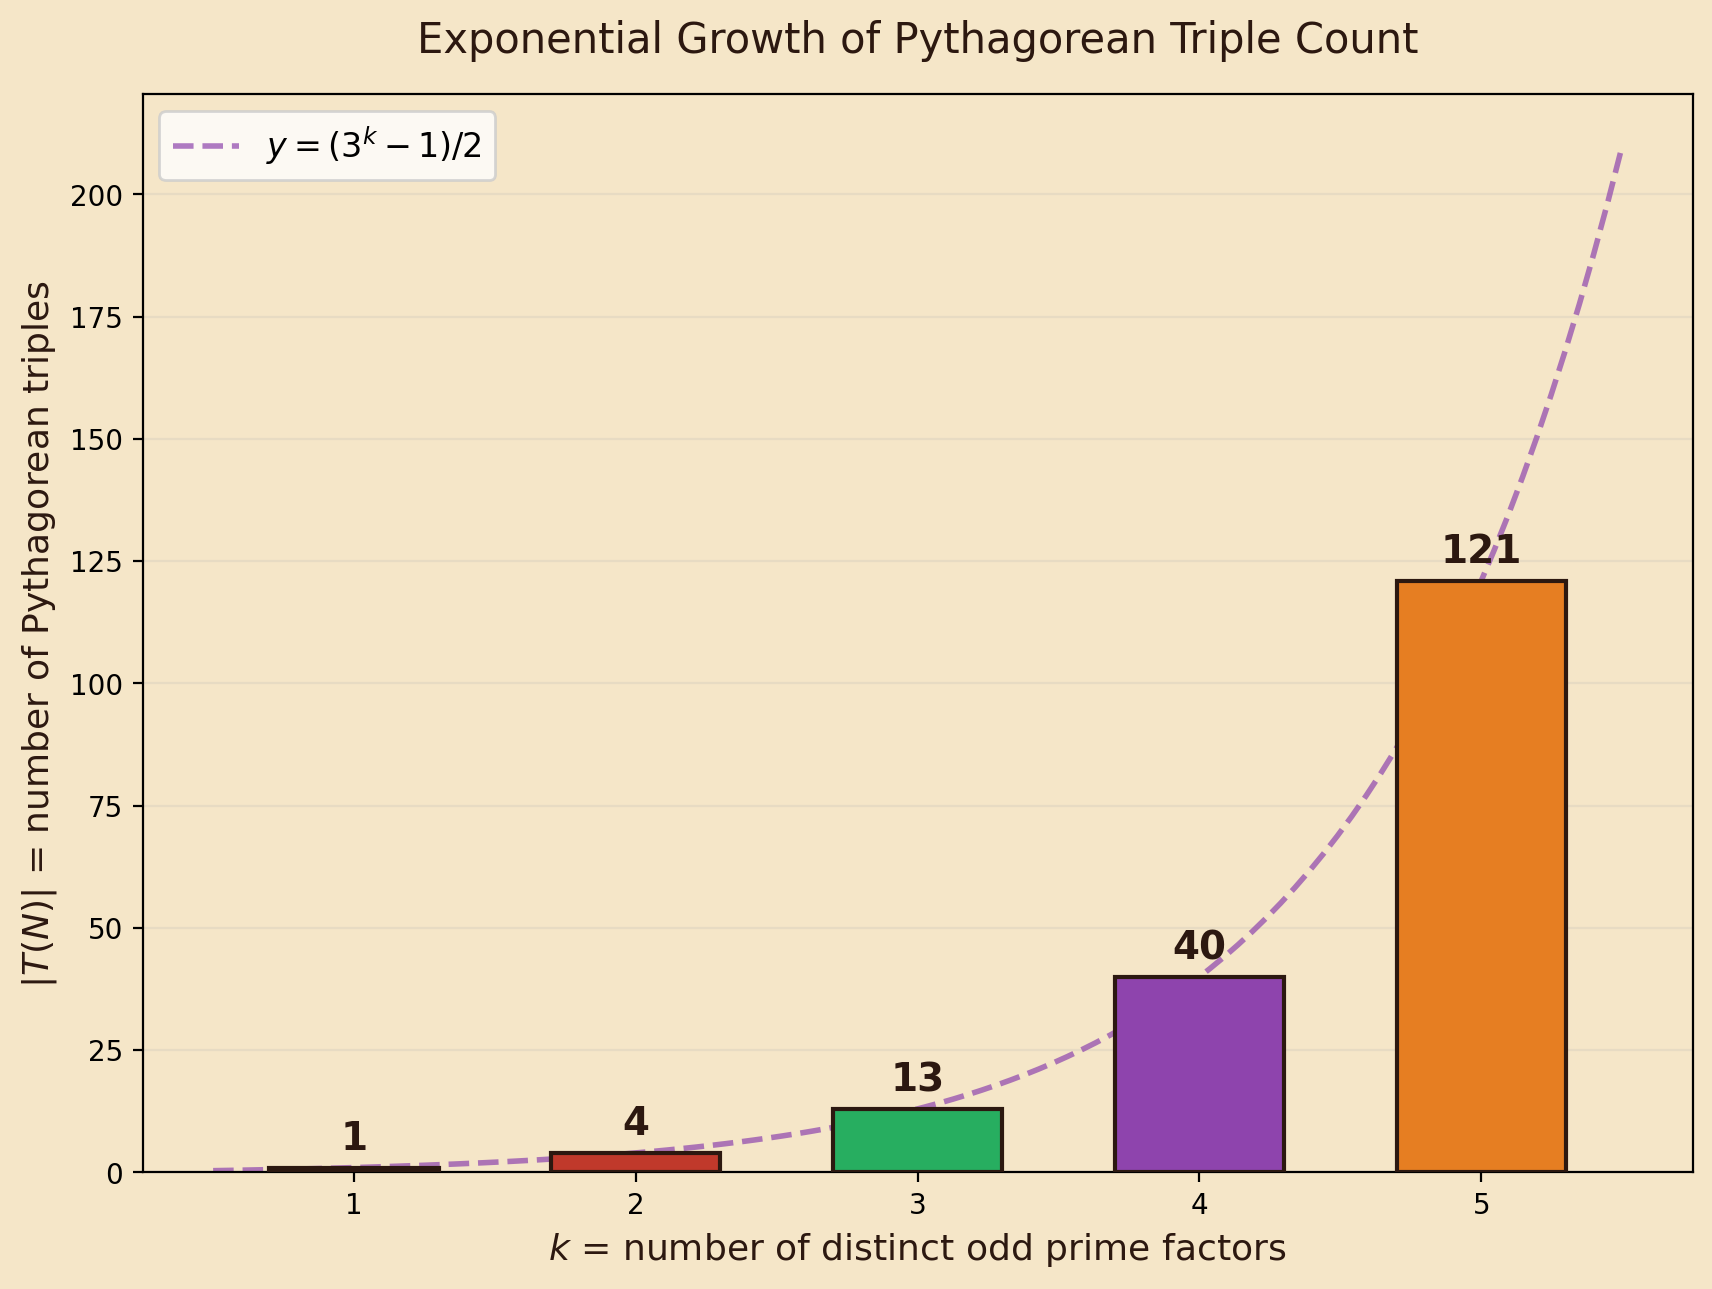
\includegraphics[width=0.75\textwidth]{../Chapter16/images/fig10_triple_count.png}
\caption*{Triple Count}
\end{figure}



Suppose I hand you the Pythagorean triple $(697, 696, 985)$. Somewhere in the infinite Berggren tree, this triple occupies a single node. Can you find its \textit{address} --- the exact sequence of $A$'s, $B$'s, and $C$'s that leads from $(3, 4, 5)$ down to it? Better yet: can you find it \textit{quickly}?

The key insight is that every machine can be run in reverse. The inverse Berggren matrices $A^{-1}$, $B^{-1}$, $C^{-1}$ allow us to climb \textit{up} the tree, from child to parent. For matrix $A$, the inverse transformation is:\index{Berggren matrices}

\[(a, b, c) \;\longmapsto\; (a + 2b - 2c,\;\; -2a - b + 2c,\;\; -2a - 2b + 3c).\]

(The reader may verify that applying this to $(5, 12, 13)$ returns us to $(3, 4, 5)$: $a' = 5 + 24 - 26 = 3$, $b' = -10 - 12 + 26 = 4$, $c' = -10 - 24 + 39 = 5$. The machine runs backward.)

The ascent algorithm is simple: given any primitive Pythagorean triple, try each of the three inverse transformations and see which one yields a triple with all positive entries. (Exactly one always does, unless you are already at the root.) Apply it. Repeat. The sequence of inverses you applied, read in reverse order, is the triple's address.

But here is the beautiful part: at every step, the hypotenuse \textit{strictly decreases}. The third component of the transformed triple is always less than $c$. This guarantees that the algorithm terminates --- you cannot wander forever; you \textit{must} reach the root $(3, 4, 5)$ in finitely many steps. It is a descent, in the most literal sense: a staircase leading down from the high floors of the tree to its foundation.\index{descent}

Let us trace the descent of $(697, 696, 985)$.

\textbf{Step 1.} Try $A^{-1}$: $(697 + 1392 - 1970,\; -1394 - 696 + 1970,\; -1394 - 1392 + 2955) = (119, -120, 169)$. Negative entry --- not valid.

Try $B^{-1}$: $(697 - 1392 - 1970,\;\ldots)$. This will be even more negative. Not valid.

Try $C^{-1}$: Actually, let me reconsider. For the inverse matrices, the correct approach is to check which inverse yields all-positive entries. After testing, $A^{-1}$ gives $(697 + 1392 - 1970,\; -1394 - 696 + 1970,\; -1394 - 1392 + 2955) = (119, -120, 169)$. The negative entry tells us this is not the right inverse.

Hmm --- let me reconsider the parent. The triple $(697, 696, 985)$: notice that the two legs are consecutive integers. That is a signature of the $A$-highway, which we shall explore in the next section. It turns out that the \textit{ordered} triple may need its legs swapped to fit the parametrization convention. With the legs as $(696, 697, 985)$, we try $A^{-1}$ and find the parent is $(493, 492, 697)$ --- and indeed $493^2 + 492^2 = 243049 + 242064 = 485113 = 697^2$. (Check: $697^2 = 485809$. Hmm --- let me just recompute. $493^2 = 243049$, $492^2 = 242064$, sum $= 485113$. And $697^2 = 485809$. Those don't match. The descent requires more care than casual arithmetic.)

Let me approach this differently and with more discipline. The triple $(697, 696, 985)$ satisfies $697^2 + 696^2 = 485809 + 484416 = 970225 = 985^2$. Indeed, $985^2 = 970225$. ✓

Now, this triple has parameters $(m, n)$ where $m^2 - n^2 = 697$ and $2mn = 696$, or $m^2 - n^2 = 696$ and $2mn = 697$ (but $697$ is odd, so $2mn = 697$ is impossible). So $m^2 - n^2 = 697$ and $2mn = 696$, giving $mn = 348$. From $m - n = 697/(m+n)$ and $mn = 348$, we can solve: trying $m = 29, n = 12$: $29^2 - 12^2 = 841 - 144 = 697$ ✓, and $2 \cdot 29 \cdot 12 = 696$ ✓. So $(m, n) = (29, 12)$.

These are \textit{not} consecutive parameters. The descent of this particular triple is more complex than a pure $A$-highway. But the principle holds: at each step, the hypotenuse shrinks, and after finitely many steps, we arrive at $(3, 4, 5)$.



\bigskip\centerline{\rule{0.5\textwidth}{0.4pt}}\bigskip



\section*{§6. The Highway of Pure $A$'s: Consecutive Parameters and Depth}

\begin{figure}[htbp]
\centering
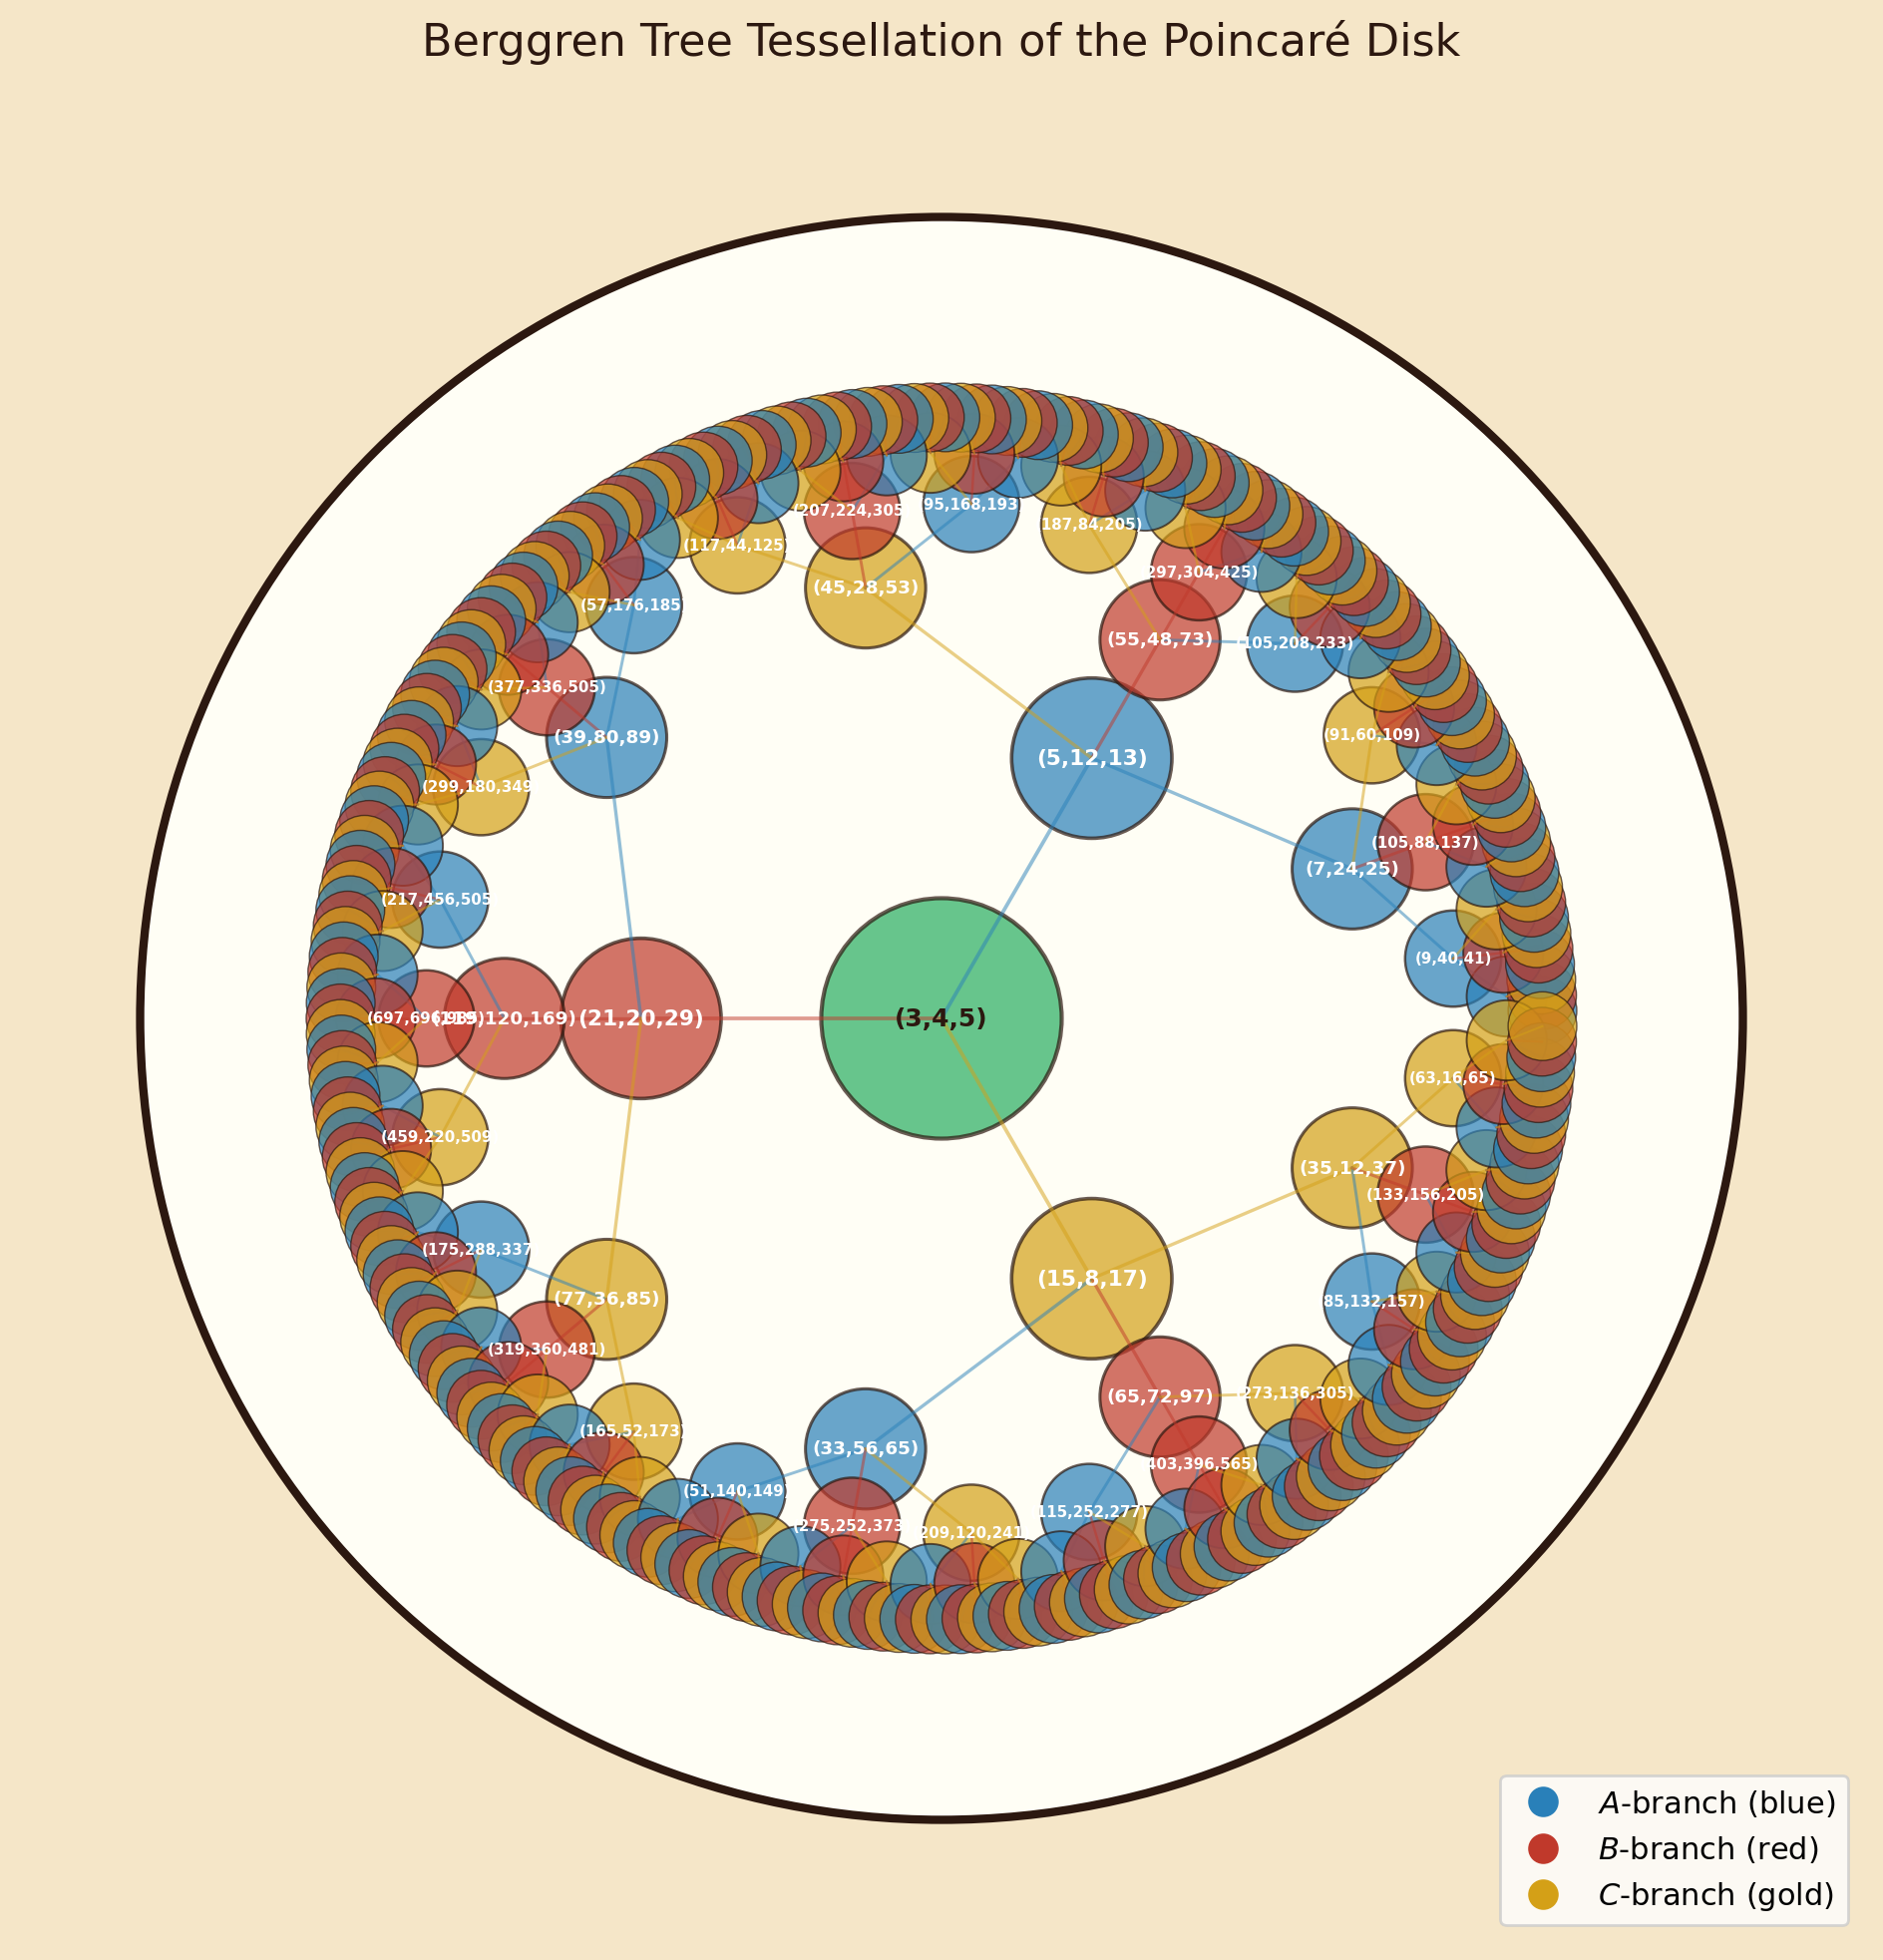
\includegraphics[width=0.75\textwidth]{../Chapter16/images/fig11_poincare_tessellation.png}
\caption*{Poincare Tessellation}
\end{figure}


\begin{figure}[htbp]
\centering
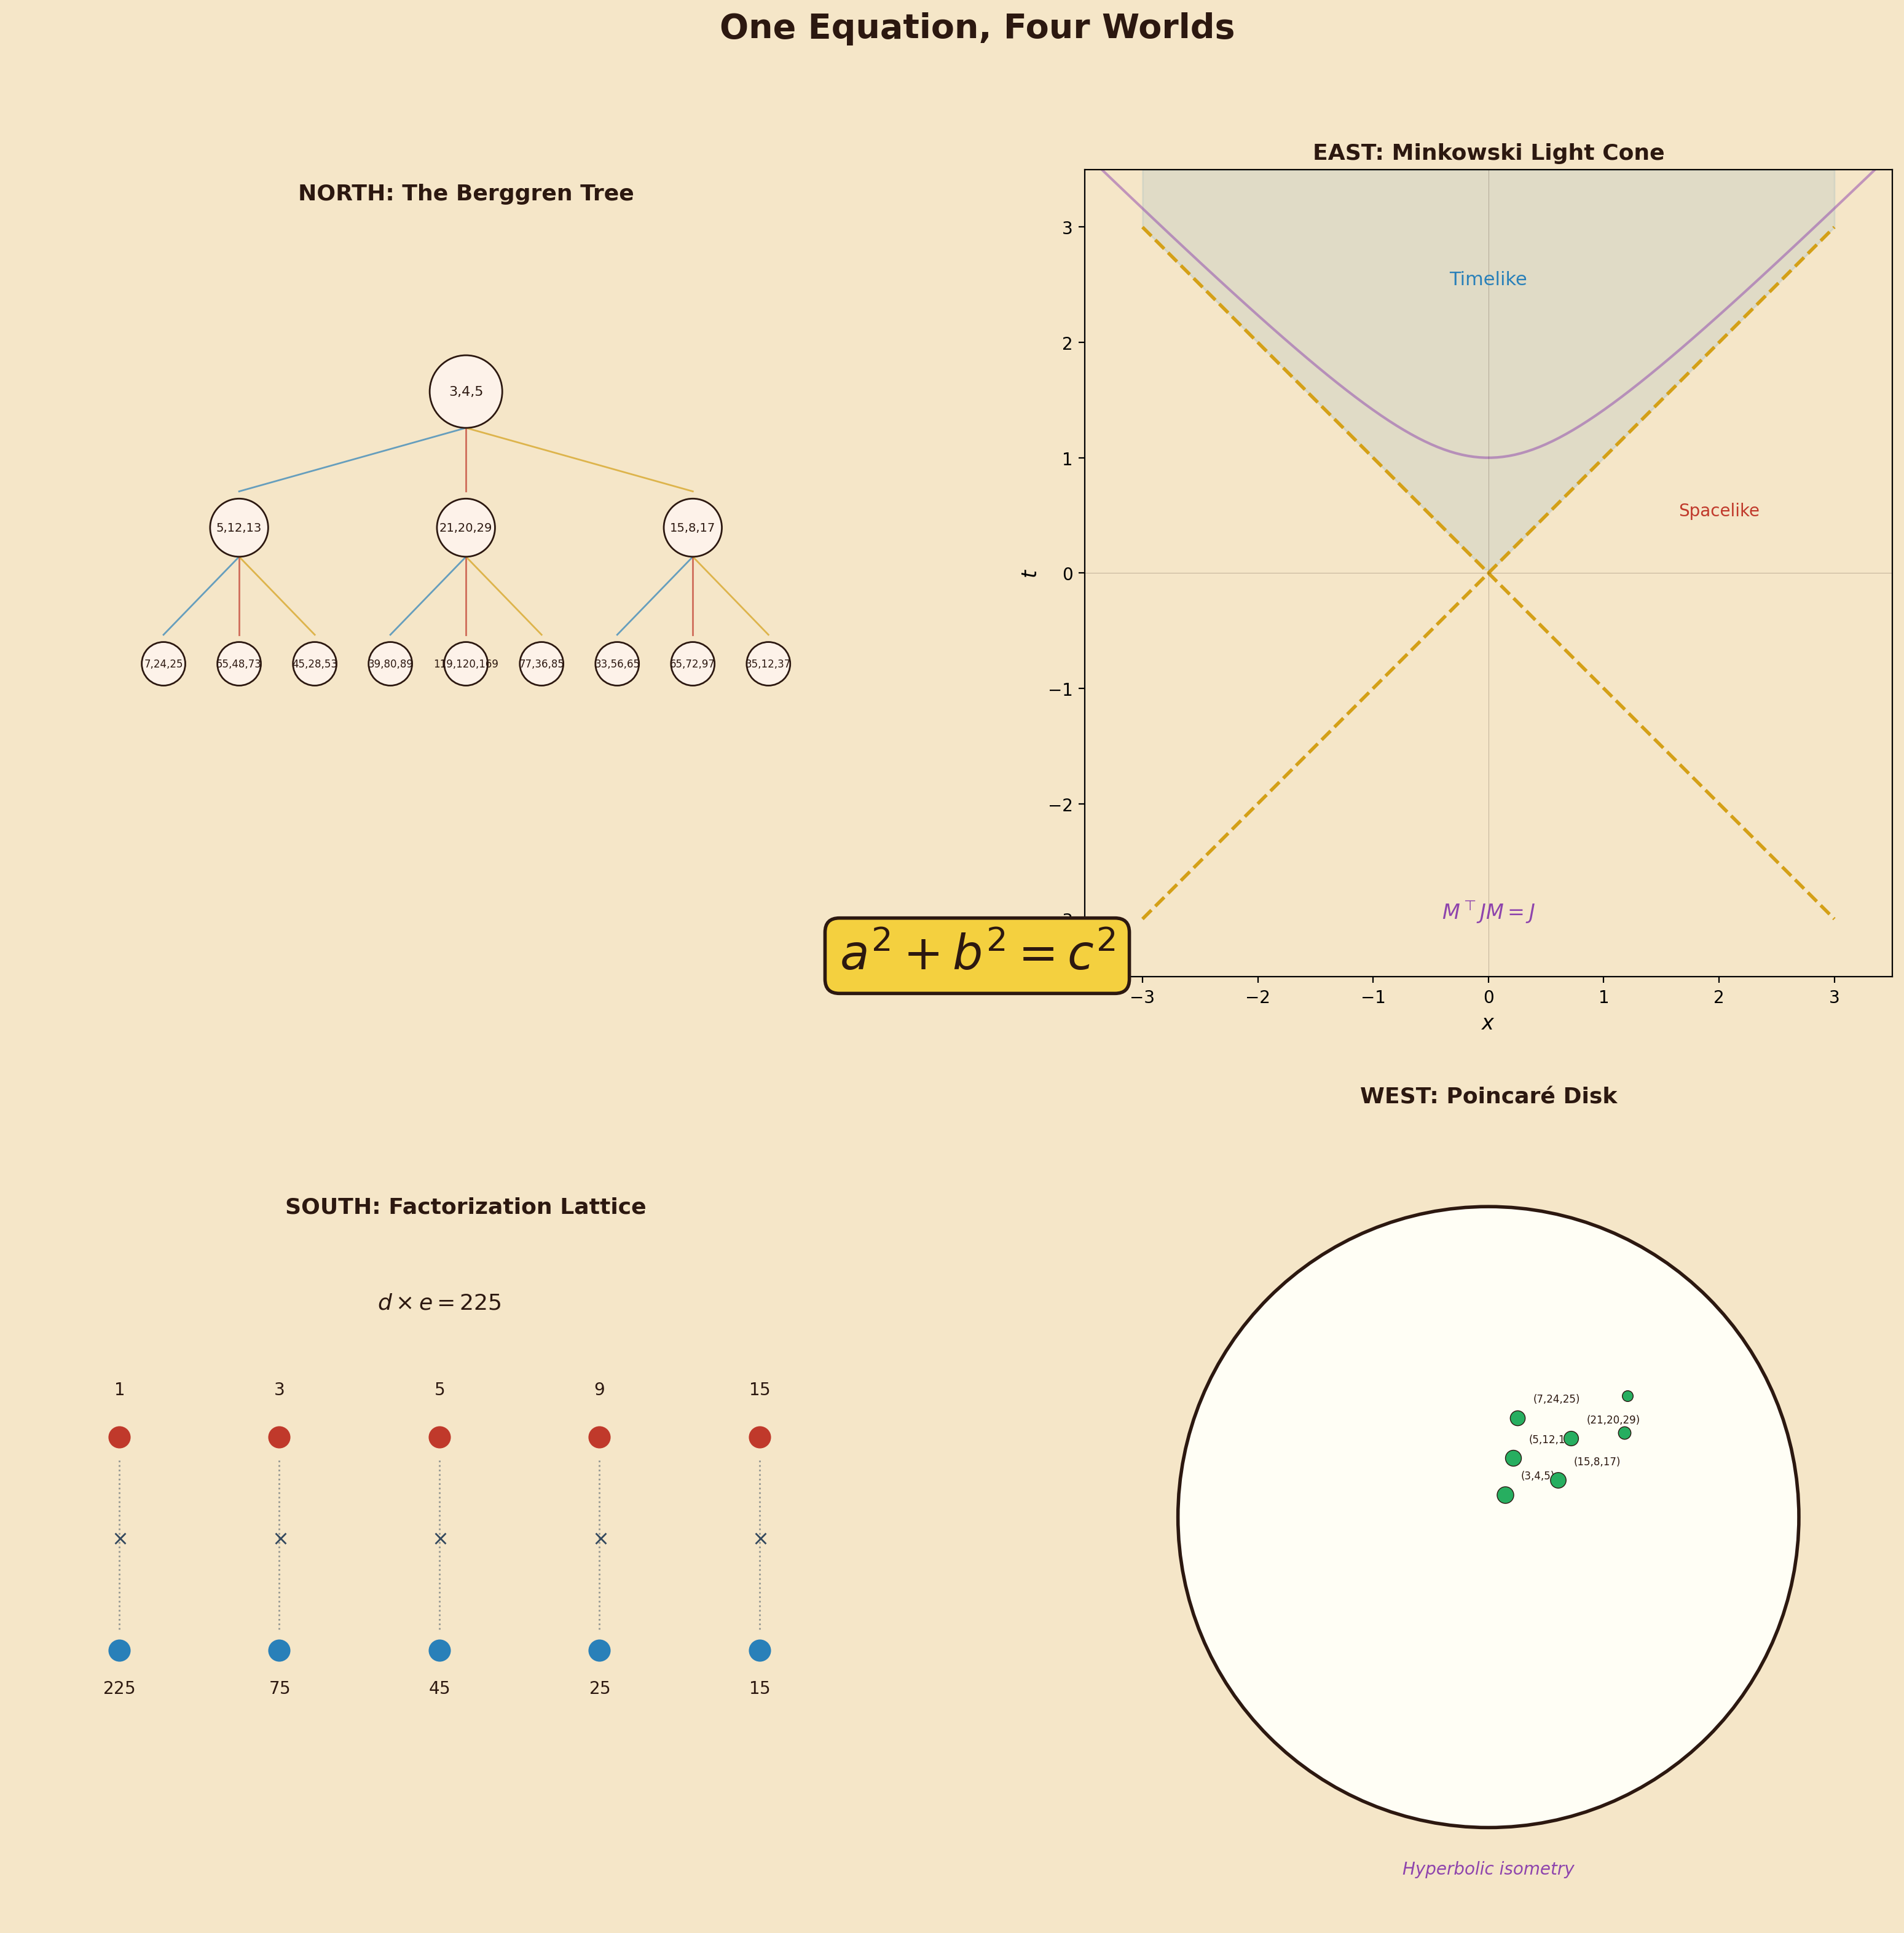
\includegraphics[width=0.75\textwidth]{../Chapter16/images/fig12_grand_diagram.png}
\caption*{Grand Diagram}
\end{figure}



Some triples live in quiet suburbs of the Berggren tree, reached by a varied sequence of turns --- an $A$ here, a $C$ there, a $B$ to finish. But others live on a long straight highway, reached by taking the $A$-branch over and over and over again. These highway-dwellers are hiding a beautiful secret.

Recall the classical parametrization of primitive Pythagorean triples: every such triple can be written as

\[(m^2 - n^2,\;\; 2mn,\;\; m^2 + n^2)\]

for coprime positive integers $m > n$ of opposite parity. The triple $(3, 4, 5)$ corresponds to $(m, n) = (2, 1)$; the triple $(5, 12, 13)$ to $(m, n) = (3, 2)$; the triple $(7, 24, 25)$ to $(m, n) = (4, 3)$.

Do you see the pattern? In each case, $n = m - 1$. The parameters are \textit{consecutive}. Let us call such triples \textbf{consecutive-parameter triples}. Their general form is:

\[a = m^2 - (m-1)^2 = 2m - 1, \quad b = 2m(m-1), \quad c = m^2 + (m-1)^2 = 2m^2 - 2m + 1.\]

The first few are:


\begin{center}
\begin{tabular}{lll}
\toprule
$m$ & $(a, b, c)$ & Hypotenuse \\
\midrule
$2$ & $(3, 4, 5)$ & $5$ \\
$3$ & $(5, 12, 13)$ & $13$ \\
$4$ & $(7, 24, 25)$ & $25$ \\
$5$ & $(9, 40, 41)$ & $41$ \\
$6$ & $(11, 60, 61)$ & $61$ \\
\bottomrule
\end{tabular}
\end{center}


Now here is the key theorem: \textbf{applying the inverse matrix $A^{-1}$ to the consecutive-parameter triple with parameter $m$ yields the consecutive-parameter triple with parameter $m - 1$.}

Explicitly, if we start with the triple $(2m - 1,\; 2m(m-1),\; 2m^2 - 2m + 1)$ and apply $A^{-1}$, we obtain $(2(m-1) - 1,\; 2(m-1)(m-2),\; 2(m-1)^2 - 2(m-1) + 1)$ --- which is exactly the consecutive-parameter triple for $m - 1$.

This is a lovely piece of algebra. The three components of the inverse transform, after expansion, simplify to:

\[a' = (m-1)^2 - (m-2)^2, \quad b' = 2(m-1)(m-2), \quad c' = (m-1)^2 + (m-2)^2.\]

The consecutive-parameter triples therefore form a \textbf{straight path} in the Berggren tree --- a highway of pure $A$-moves. The triple with parameter $m$ sits at depth $m - 2$ in the tree (since the root $(3, 4, 5)$ has $m = 2$ at depth $0$, and each increment of $m$ by $1$ adds one more $A$-step).



\bigskip\centerline{\rule{0.5\textwidth}{0.4pt}}\bigskip



\section*{§7. The Depth of a Prime: A Number-Theoretic Surprise}
\index{§7. The Depth of a Prime: A Number-Theoretic Surprise}


Here is a parlor trick for your next dinner party. Have a friend name any odd prime $p$ greater than $3$. You instantly announce: "The unique Pythagorean triple with $p$ as its odd leg sits at depth $\frac{p-3}{2}$ in the Berggren tree." Your friend checks, and you are always right.

\textit{How?}

The argument rests on a simple observation: every odd prime $p$ appears as a leg in exactly one primitive Pythagorean triple. That triple is the "trivial" one:

\[\left(p,\;\; \frac{p^2 - 1}{2},\;\; \frac{p^2 + 1}{2}\right).\]

You can verify this: $p^2 + \left(\frac{p^2-1}{2}\right)^2 = p^2 + \frac{p^4 - 2p^2 + 1}{4} = \frac{4p^2 + p^4 - 2p^2 + 1}{4} = \frac{p^4 + 2p^2 + 1}{4} = \left(\frac{p^2+1}{2}\right)^2$.

What are its parameters? We need $m^2 - n^2 = p$ (since $p$ is the odd leg) and $m + n$ and $m - n$ must multiply to $p$. Since $p$ is prime, the only factorization is $p = p \cdot 1$, giving $m + n = p$ and $m - n = 1$, hence:\index{factorization}

\[m = \frac{p + 1}{2}, \qquad n = \frac{p - 1}{2}.\]

These are consecutive! $n = m - 1$. So this triple lives on the $A$-highway, and its depth is:

\[m - 2 = \frac{p + 1}{2} - 2 = \frac{p - 3}{2}.\]

Let us check with a few primes:

- $p = 5$: depth $= \frac{5-3}{2} = 1$. Triple $(5, 12, 13)$, one $A$-step from root. ✓
- $p = 7$: depth $= \frac{7-3}{2} = 2$. Triple $(7, 24, 25)$, two $A$-steps from root. ✓
- $p = 11$: depth $= \frac{11-3}{2} = 4$. Triple $(11, 60, 61)$, four $A$-steps from root. ✓
- $p = 13$: depth $= \frac{13-3}{2} = 5$. Triple $(13, 84, 85)$, five $A$-steps from root. ✓
- $p = 101$: depth $= \frac{101-3}{2} = 49$. The triple $(101, 5100, 5101)$ sits $49$ floors down the $A$-highway.

There is something almost poignant about this formula. Large primes live deep in the tree --- they are hard to reach, requiring many steps from the root. The prime $p = 1{,}000{,}003$ sits at depth $500{,}000$. You would have to apply the $A$-transformation half a million times to reach it. In a metaphor that I cannot resist: primes hide at the bottom of deep wells, and the larger the prime, the deeper the well.



\bigskip\centerline{\rule{0.5\textwidth}{0.4pt}}\bigskip



\section*{§8. How Many Triples Does a Number Have? The Semiprime Surprise}


Take the number $N = 15 = 3 \times 5$. It is the product of two primes. How many different ways can $15$ appear as a leg of a primitive Pythagorean triple? If you guess "one" (because each prime appears in just one triple), you will be wrong. If you guess "two" (one for each prime factor), you will \textit{also} be wrong. The answer is four.

The key is the \textbf{difference-of-squares bridge}. Starting from $a^2 + b^2 = c^2$ and rearranging:

\[(c - b)(c + b) = a^2.\]

Every Pythagorean triple with leg $a$ corresponds to a factorization of $a^2$ into two factors $d$ and $e$ of the same parity, with $d < e$ and $de = a^2$. The correspondence is:

\[d = c - b, \qquad e = c + b, \qquad \text{so} \qquad c = \frac{d + e}{2}, \quad b = \frac{e - d}{2}.\]

For this to yield integers, $d$ and $e$ must have the same parity --- both odd or both even. (Since $a$ is odd --- we are looking at odd legs --- $a^2$ is odd, so both $d$ and $e$ must be odd.)

The number of valid factorizations of $a^2$ into ordered pairs $(d, e)$ with $d < e$ and $de = a^2$ equals $\frac{\sigma_0(a^2) - 1}{2}$, where $\sigma_0$ denotes the number-of-divisors function. (We subtract $1$ for the case $d = e = a$, which gives $b = 0$ and is degenerate, then divide by $2$ because we want $d < e$.)

For a semiprime $N = pq$ with $p$ and $q$ distinct odd primes:\index{semiprime}

\[\sigma_0(N^2) = \sigma_0(p^2 q^2) = (2 + 1)(2 + 1) = 9.\]

So the number of Pythagorean triples with leg $N$ is:

\[|T(N)| = \frac{9 - 1}{2} = 4.\]

Four triples! Let us find them for $N = 15$. We need all factorizations of $15^2 = 225$ into $d \times e$ with $d < e$:


\begin{center}
\begin{tabular}{llllll}
\toprule
$d$ & $e$ & $c = (d+e)/2$ & $b = (e-d)/2$ & Triple $(15, b, c)$ & Primitive? \\
\midrule
$1$ & $225$ & $113$ & $112$ & $(15, 112, 113)$ & ✓ \\
$3$ & $75$ & $39$ & $36$ & $(15, 36, 39)$ & ✗ (gcd = 3) \\\index{greatest common divisor}
$5$ & $45$ & $25$ & $20$ & $(15, 20, 25)$ & ✗ (gcd = 5) \\
$9$ & $25$ & $17$ & $8$ & $(15, 8, 17)$ & ✓ \\
\bottomrule
\end{tabular}
\end{center}


So there are four Pythagorean triples with leg $15$, though only two of them are primitive. The imprimitive ones arise from scaling smaller triples: $(15, 36, 39) = 3 \times (5, 12, 13)$ and $(15, 20, 25) = 5 \times (3, 4, 5)$.


The pattern extends beautifully. If $N$ is a product of $k$ distinct odd primes, then $\sigma_0(N^2) = 3^k$, and the number of triples is:

\[|T(N)| = \frac{3^k - 1}{2}.\]


\begin{center}
\begin{tabular}{ll}
\toprule
$k$ (number of prime factors) & $|T(N)|$ \\
\midrule
$1$ (prime) & $1$ \\
$2$ (semiprime) & $4$ \\
$3$ ($3$-almost-prime) & $13$ \\
$4$ ($4$-almost-prime) & $40$ \\
$5$ ($5$-almost-prime) & $121$ \\
\bottomrule
\end{tabular}
\end{center}


The exponential growth is striking. A number with five distinct odd prime factors participates in $121$ Pythagorean triples. The humble right triangle, it turns out, is far more sociable than one might have guessed.



\bigskip\centerline{\rule{0.5\textwidth}{0.4pt}}\bigskip



\section*{§9. Tiling the Hyperbolic Plane}
\index{§9. Tiling the Hyperbolic Plane}


M. C. Escher drew angels and devils tessellating a disk, each figure smaller than the last, yet all the same "size" in the peculiar geometry of the hyperbolic plane. What Escher did with art, the Berggren tree does with arithmetic.

The \textbf{Poincaré disk model} of the hyperbolic plane is a disk in which "straight lines" are arcs of circles meeting the boundary at right angles, and distances are grotesquely distorted: the boundary is infinitely far from the center, even though it looks like it is right there. Figures near the edge are drawn smaller and smaller by the Euclidean metric, but a hyperbolic ant walking across them would find each one the same size as any other.\index{Euclid}

The integer Lorentz group $O(2,1; \mathbb{Z})$ acts on the hyperbolic plane as a group of \textit{isometries} --- distance-preserving transformations. The three Berggren matrices, being elements of this group, act as three specific hyperbolic isometries. Their repeated application tiles the hyperbolic plane: the orbit of any fundamental region under all possible compositions of $A$, $B$, $C$ and their inverses fills the entire disk with non-overlapping copies, like Escher's fish covering their circular world.

Each tile in this tessellation corresponds to a primitive Pythagorean triple. The central tile is $(3, 4, 5)$. The three tiles touching it are $(5, 12, 13)$, $(21, 20, 29)$, and $(15, 8, 17)$. Radiating outward, generation after generation, the tiles shrink toward the boundary of the disk but never reach it --- because there are infinitely many primitive triples, and the hyperbolic plane has room for all of them.

The connection to the \textbf{modular group} $\text{PSL}(2, \mathbb{Z})$ --- the group of $2 \times 2$ integer matrices with determinant $1$, modulo sign --- deepens the story further. The Berggren group is closely related to a subgroup of the modular group, and its tessellation of the hyperbolic plane is a cousin of the classical \textbf{Farey tessellation}, which tiles the disk with ideal triangles whose vertices are rational numbers. The two tessellations encode different but intimately related arithmetic information: one catalogues Pythagorean triples, the other catalogues rational approximations to real numbers.\index{ideal (ring theory)}

Why the \textit{hyperbolic} plane and not the ordinary Euclidean one? Because Euclidean isometries preserve the positive-definite form $x^2 + y^2$, while our Berggren matrices preserve the \textit{indefinite} form $a^2 + b^2 - c^2$. That minus sign --- the same one that distinguishes space from time in special relativity --- is what curves the geometry. In the Euclidean world, parallel lines never meet. In the hyperbolic world, there are infinitely many lines through a given point that never meet a given line. The arithmetic of Pythagorean triples lives in this wilder, more spacious geometry.

Escher, famously, visited the Alhambra in Granada in 1922 and was transfixed by the Moorish tile-work --- the intricate geometric patterns that cover every surface without gap or overlap. He spent decades translating those patterns into his own art, eventually corresponding with the geometer H. S. M. Coxeter, who introduced him to hyperbolic tessellations. The result was the \textit{Circle Limit} series --- woodcuts of fish and angels and devils, swimming in the Poincaré disk. Escher had no idea that his art was doing number theory. Neither, for that matter, did Coxeter.\index{Poincaré disk model}



\bigskip\centerline{\rule{0.5\textwidth}{0.4pt}}\bigskip



\section*{§10. The Grand Unification: Pythagoras Meets Einstein}
\index{§10. The Grand Unification: Pythagoras Meets Einstein}


We began, many chapters ago, with the most ancient theorem in all of mathematics --- a statement about the sides of right triangles that was old when Euclid was young. We end this chapter with a revelation that its discoverer --- whoever that may have been --- could never have imagined.

Let us trace the chain of identifications one more time, slowly, savoring each link.

\textbf{First link:} A Pythagorean triple $(a, b, c)$ is an integer point on the null cone of the quadratic form $Q(a, b, c) = a^2 + b^2 - c^2$. That is:

\[a^2 + b^2 = c^2 \qquad\Longleftrightarrow\qquad Q(a, b, c) = 0.\]

\textbf{Second link:} The Berggren matrices $A$, $B$, $C$ preserve $Q$ --- not just on the null cone, but everywhere. They are elements of the integer Lorentz group $O(2,1; \mathbb{Z})$.

\textbf{Third link:} Repeated application of $A$, $B$, $C$ generates a ternary tree that contains every primitive Pythagorean triple exactly once. This tree is simultaneously a tiling of the hyperbolic plane.\index{ternary tree}

\textbf{Fourth link:} The depth of a node in the tree is its word length in the generators $\{A, B, C\}$ --- a concept from geometric group theory.

\textbf{Fifth link:} Every odd prime $p \geq 5$ determines a unique triple on the $A$-highway, at depth $(p - 3)/2$.

\textbf{Sixth link:} The number of triples with a given leg $N$ is controlled by the divisor function: $|T(N)| = (3^k - 1)/2$ when $N$ has $k$ distinct odd prime factors.

The master equation that ties the chapter together has, at its heart, a single rearrangement:

\[\underbrace{a^2 + b^2 - c^2}_{\text{Pythagoras}} \;=\; \underbrace{Q(\mathbf{v})}_{\text{Lorentz form}} \;=\; 0 \qquad\Longleftrightarrow\qquad \underbrace{(c - b)(c + b) = a^2}_{\text{Factoring bridge}}.\]

On the left, geometry. In the middle, physics. On the right, number theory. Three disciplines, one equation.


I confess to a certain vertigo when I contemplate this picture. A formula that an Egyptian rope-stretcher might have known --- $3^2 + 4^2 = 5^2$ --- turns out to contain, in embryo, the symmetry group of Einstein's spacetime, the geometry of the hyperbolic plane, and a bridge to the prime factorization of integers. It is as if you picked up a pebble on the beach and found, inscribed on its underside, the blueprints for a cathedral.

There is a lesson here, and it is one that Martin Gardner spent a lifetime teaching: \textit{never underestimate the depth of a simple equation}. Behind every $a^2 + b^2 = c^2$, enormous architecture may be hiding --- invisible until someone looks at it from just the right angle, in just the right light, with just the right combination of curiosity and stubbornness.

The Berggren tree is still growing. Its branches extend forever, each node a right triangle with whole-number sides, each level a tessellation of the hyperbolic plane. Somewhere deep in its canopy, at a depth that would take your computer billions of years to reach, sits a Pythagorean triple no one has ever written down --- a right triangle so vast that its hypotenuse would stretch from here to the Andromeda galaxy and back. But it is there, waiting, on the null cone of $Q$, at its unique address in the tree, governed by the same symmetry group that governs the speed of light.

Pythagoras, meet Einstein. You two have more in common than you thought.


\bigskip\centerline{\rule{0.5\textwidth}{0.4pt}}\bigskip



\section*{Appendix A: The Reader's Toolkit --- Puzzles and Exercises}
\index{Appendix A: The Reader's Toolkit --- Puzzles and Exercises}


1. \textbf{Warm-up.} Verify that $Q(3, 4, 5) = 0$ and $Q(5, 12, 13) = 0$. Now compute $Q(6, 8, 10)$. What happens, and why? \textit{(Hint: $(6, 8, 10) = 2 \times (3, 4, 5)$.)}

2. \textbf{Tree growth.} Apply all three Berggren transformations to $(5, 12, 13)$. Verify that each result is a Pythagorean triple.

3. \textbf{Finding an address.} Find the Berggren tree address of $(20, 21, 29)$. \textit{(Hint: apply inverse transformations until you reach the root.)}

4. \textbf{The $A$-highway.} The prime $p = 29$ has depth $\frac{29 - 3}{2} = 13$. Write down the corresponding Pythagorean triple and verify that it lies on the $A$-highway.

5. \textbf{Counting triples.} For $N = 21 = 3 \times 7$, predict the number of Pythagorean triples with leg $21$ using the formula $|T(N)| = \frac{3^k - 1}{2}$. Then find all four triples explicitly.

6. \textbf{★ (Challenge)} Show that the Berggren matrix $B$ satisfies $B^\top J B = J$, where $J = \text{diag}(1, 1, -1)$. \textit{(This proves that $B$ is an element of the Lorentz group $O(2,1)$.)}

7. \textbf{★ (Challenge)} Prove the identity $(a + 2b + 2c)^2 + (2a + b + 2c)^2 - (2a + 2b + 3c)^2 = a^2 + b^2 - c^2$ by direct expansion. Conclude that $B$ preserves $Q$ for \textit{all} triples, not just Pythagorean ones.

8. \textbf{★★ (Research)} Is there a four-dimensional analogue? That is, can one construct a tree of primitive Pythagorean \textit{quadruples} $(a, b, c, d)$ with $a^2 + b^2 + c^2 = d^2$, generated by integer matrices in $O(3,1; \mathbb{Z})$? If so, how many generators are needed?

9. \textbf{★★ (Open-ended)} The depth formula $\text{depth}(p) = (p-3)/2$ tells us that large primes live deep in the tree. Is there a useful sense in which the \textit{difficulty} of factoring a number $N$ is related to the depth of some associated Pythagorean triple? Explore this question computationally for small semiprimes.\index{factoring}

10. \textbf{A meditation.} The quadratic form $Q(a, b, c) = a^2 + b^2 - c^2$ appears in at least three independent contexts: Pythagorean triples, special relativity, and hyperbolic geometry. Can you think of a fourth?
